%Template by Mark Jervelund - 2015 - mjerv15@student.sdu.dk

\documentclass[a4paper,10pt,titlepage]{report}

\usepackage[utf8]{inputenc}
\usepackage[T1]{fontenc}
\usepackage[english]{babel}
\usepackage{amssymb}
\usepackage{amsmath}
\usepackage{amsthm}
\usepackage{graphicx}
\usepackage{fancyhdr}
\usepackage{lastpage}
\usepackage{listings}
\usepackage{algorithm}
\usepackage{marvosym}
\usepackage{algpseudocode}
\usepackage[document]{ragged2e}
\usepackage[margin=1in]{geometry}
\usepackage{color}
\usepackage{datenumber}
\usepackage{venndiagram}
\usepackage{chngcntr}
\usepackage[utf8]{inputenc}
\usepackage[english]{babel}
\usepackage{amssymb,amsmath,amsthm}
\usepackage{mathtools}
\usepackage{wrapfig}
\usepackage{multirow}
\usepackage{mathtools} % Bonus
\usepackage[
    backend=biber,
    style=numeric,
    sorting=ynt
]{biblatex}

\newtheorem{theorem}{Theorem}



\addbibresource{bibliography.bib}


\DeclarePairedDelimiter\norm\lVert\rVert
\setdatetoday
\addtocounter{datenumber}{0} %date for dilierry standard is today
\setdatebynumber{\thedatenumber}
\date{}
\setcounter{secnumdepth}{0}
\pagestyle{fancy}
\fancyhf{}
\title{Masters Thesis}

\newcommand{\Z}{\mathbb{Z}}
\lhead{Masters Thesis}
\rhead{Mark Jervelund}
\rfoot{Page  \thepage \, of \pageref{LastPage}}
\counterwithin*{equation}{section}

\begin{document}
\begin{titlepage}
\centering
    \vspace*{9\baselineskip}
    \huge
    \bfseries
    Jepsen methods usage for ACID compliance in Hyperscale Cloud Frameworks \\
    \normalfont
    Mark Jervelund \\
    Mark@jervelund.com \\
    \vspace*{9\baselineskip}
    \normalfont
	
\includegraphics[scale=1]{logos/SDU_BLACK.png}
    \vfill\
    \vspace{5mm}
    Institute Of Mathematics and Computer Science, SDU \\

	%Date
    \textbf{\datedate} \\[2\baselineskip]
\end{titlepage}

\renewcommand{\thepage}{\roman{page}}% Roman numerals for page counter
\tableofcontents
\newpage
\setcounter{page}{1}
\renewcommand{\thepage}{\arabic{page}}


\section*{Abstract}

Databases allow modern society to store, manage and distribute data at a previously unprecedentedly scale, having data is a normal practice for most businesses, but it is often done monotonically on a single node, where modern needs require much high performance, storage, latency and  availability then current systems allow. Distributing a data store in a manner that scales performance, storage, availability and desire properties is no easy feat. In this Thesis i present methods of verifying these properties and investigate how different frameworks solve this issue, or often workaround the issue in a way that aligns with the requirements of the systems. \\
\vspace{5mm}

Within the framework of the thesis i present methods of verifying the ACID properties, How these properties were solved in the past, How it can and is solved today, what trade offs some systems have made, and a analysis of modern database uses cases and whether they require the ACID properties to solve issues.\\
\vspace{5mm}

Summarize the findings and try to say why the thesis is worth reading.



\chapter{Introduction}

Highly Distributed systems are becoming more and more common as the world grows evermore interconnected, faster paced, increasing data driven with higher expectations of services and product. where the end user expects reliability, availability combined with low- latency and cost, How do we guarantee this is a distributed system that spans the planet. Is it even possible to get both, and is it even needed in most use cases?\\
\vspace{5mm}
Most people are familiar with how YouTube, Facebook, Google and Reddit behave. What quirks they sometimes present, Most people remember the YouTube video counter that got stuck around 300, and didn't update for a while, The reason it got stuck was induced, however the number it got stuck on was not, The system was designed to stop at 301, but often went higher. This is an example of the system not being entirely consistent, most nodes where in the correct state of stopping counting when the number got larger then 300, however as some nodes around the globe weren't in an consistent state these still counted the views onto the displayed counter when they were supposed to have been sent to a different table that verified the views before considering them legitimate. This number is still not consistent around the world however for human use cases the issue of a comment or view being a few seconds or ½ a minute delayed isn't something we notice or care about. a lot of user facing services aren't required to be ACID compliant, however there are use cases where this can have an impact is when dealing with data that is produced and consumed in real time, if this is finance, automated or autonomous systems, or other areas where having consistent, atomic and isolated transactions are of the utmost importance. these cases are where it doesn't matter what server we are querying the information from it has to be the most recent sample, and if we at any point are able to query stale data we end up being at the risk of either making an illegal transaction or an autonomous system making a wrong decision, This can a trading system fetching stale data and making the wrong transaction, a bank withdrawal that might be overdrawing the users account. or autonomous vehicle that might making decisions with stale data that can lead to fatal accidents. \\
\vspace{5mm}
How do we test and verify that the systems that handle tasks that require compliance with ACID also do so. To understand this we first need to understand the basis for and expected behavior of ACID and the different levels of each of the properties of ACID.
\\

 First, I Present ACID \& Base, their constraints, what faults occur in database systems, how their manifests themselves, whats the underlying causes often are, and what limits the ACID properties imposes on a given system. Here Base will be introduced to explain what relaxations are introduced to a system where gaining the desire results for certain use cases. \\
\vspace{5mm}
Then, I Present Jepsen, a CLojure framework\cite{jepsonio} developed by K. Kingsbury that allow for testing of distributed systems, This is solved via a direct serialization graph (DSG) and queries to the target system that are carefully chosen that allows for traceability, and recoverability.  \\
\vspace{5mm}

Then, I present Azure Service Fabric(SF), SF is a distributed container orchestration system made my Microsoft, that allows for hosting of services, or apps. It includes a few different built in functions, but the primary interest here lie within the reliable containers aspect of SF, and what claims Microsoft makes concerning the behavior of this data.\\
\vspace{5mm}
Then, I will present what modern database systems promise, what properties of ACID they follow, which they relax, and which they disregard, and well as what they gain, and which tradeoffs they suffer, Here a main focus will be on Service Fabric.\\
\vspace{5mm}
Then I will present the attempt to implement and execute a Jepsen test against service Fabrics reliable containers, and compare these results to the claims Microsoft has made.\\
\vspace{5mm}
Finally, I will present how the ACID properties compare to modern uses cases of databases, do we need to follow them strictly or can simply disregard them in some uses cases? What are the exceptions, and what is there to gain ?\\

\chapter{Database transaction models}

Database and data store models can be categories into two main groups, ACID and BASE. Consistent or available. The underlying reason for this limitation is either latency between nodes in a system, scale-ability both in terms of storage or Capacity in terms of queries to the system. Both models of designing the system has it's trade-offs which will be presented later in the paper.
\section{ACID}

The ACID Model of handling database transactions is considered monolithic by some, however they still serve a vital a critical function for handling critical systems that require atomicity, consistency across the entire data-set, reliability, and durability.\\
\vspace{5mm}
The ACID acronym is defined as follows in the DBMS book\cite{DBMSbook}.

\begin{itemize}
    \item “A” stands for “atomicity,” the all-or-nothing execution of transactions.
    \item “C,” stands for “consistency.” That is, all databases
have consistency constraints, or expectations about relationships among
data elements (e.g., account balances may not be negative after a transaction finishes). Transactions are expected to preserve the consistency of
the database.
\item “I” stands for “isolation,” the fact that each transaction must appear
to be executed as if no other transaction is executing at the same
time.
\item “D” stands for “durability,” the condition that the effect on the
database of a transaction must never be lost, once the transaction
has completed.
\end{itemize}

ACID therefor offers strong consistency with rigorous handling of transaction isolation that prevent inaccurate data. This allows for designing of a system, where we can prevent operations on stale data, data loss, or "illegal" transactions. These faults will be presented further down in the paper.


\section{BASE}
The BASE model allows designing of a system where we value availability, throughput and scale-ability. This can cause issues with stale data, dirty reads, overwriting data, and other undesired behavior. This can benefit some applications where overwriting old data isn't an issue or where the newest version of data might not be required as long as it'll come eventually. The use for these databases are hugely beneficial for social media, logging, and other hyperscale system where consistency isn't required.\\
\vspace{5mm}
The Base Acronym was defined by Eric Brewer\cite{brewer2000towards} and is defined as follows.

\begin{itemize}
    \item Basically Available – Rather than enforcing immediate consistency, BASE-modelled NoSQL databases will ensure availability of data by spreading and replicating it across the nodes of the database cluster.
    \item Soft State – Due to the lack of immediate consistency, data values may change over time. The BASE model breaks off with the concept of a database which enforces its own consistency, delegating that responsibility to developers.
    \item Eventually Consistent – The fact that BASE does not enforce immediate consistency does not mean that it never achieves it. However, until it does, data reads are still possible (even though they might not reflect the reality).
\end{itemize}

The BASE model of databases often have a weak consistency where stale data is considered "OK" so to say, while offering a best effort approach with approximate answers. but gains availability, performance, and it can be considered a relaxed way of handing the database side of things where the system database system is simpler and easier to modify the schema..

\section{CAP theorem}

The CAP Theorem was defined by Eric Brewer\cite{CAP} where it states that it is impossible for a distributed database system to provide Consistency, Availability, and Partition Tolerance in a single system, and that only two of these guarantees can be met.\\
\vspace{5mm}
It should be noted that the definitions of the terms differ from the definitions in ACID. They are all important when it comes to a distributed systems and their behaviors. firstly Consistency in ACID is define as constraints on the data. By the CAP consistency concept, ACID would follow Sequential consistency as defined by Lamport\cite{lamport1993how}: “the program behaves as if the memory accesses of all processes were interleaved and then executed sequentially.” while the consistency model in CAP is defined as Atomic Consistency (also called linearizability) is sequential plus a real-time constraint: “Unlike sequential consistency, linearizability implicitly assumes the notion of an observable global time across all processes. Operations are modeled by an interval which consists of the period of time between the invocation and response for the operation and each operation is assumed to take effect instantaneously at some point within this interval.” \cite{CSL-TR-95-685}
\vspace{5mm}
CAP states we can only have 2 of the 3 properties in any given data-share system. The three different options will be explained below.
\begin{itemize}
\item Consistency and Partition tolerance(CP) \\ A system that deliveries Consistency and Partition tolerance but the trade off here is Availability, If a partition occurs in the system, the non-consistent nodes would have to be shut down or made unavailable to deliver consistent data. CP would cover majority protocols, and most distributed databases. an Example of a CP database would be MongoDB and Service Fabrics Reliable collections, These work by having partitions that contain a master and a set of replicates. The replicates simple follow the masters transaction log and apply it to their own data set. If the Primary becomes unavailable the Replicate with the most recent transaction log simply comes the new Master, doing this switch the partition becomes unavailable while the replicates catches up to the new master. this causes the network to remain consistent but limits availability.  \\

\item Availability and Partition tolerance (AP) \\ If our system foregoes Consistency, and deliverers availability and partition tolerance, In the case of a partition between nodes we keep serving from all nodes but in this case we might serve stale data and occurrence might also occur where the same row contains different values due to multiple different write operations on the different nodes. An example of a AP database would be Cassandra, where the CP have a master/replicate architecture, This would cover DNS, Caching systems and databases such as Cassandra. Cassandra uses a leaderless architecture, It does mean that there is multiple points of failure rather then a single one. It is able to be available and partition tolerant but consistency isn't guaranteed as nodes are always available and in case of partitioning the nodes will diverge when partitions and will then heal once they are connected back to the network.   \\

\item Availability and Consistency (CA) \\ Database delivers consistency and availability but doesn't allow for partitions of the network or nodes. this results in a single node, or single cluster system as any distribution of the system introduces network instability and latency that would break the system. In this case it would cover single node/site databases and cluster databases as well as file systems as we in practice wouldn't have a distributed system that doesn't allow for partitioning as it would be unusable. But an example of this would be a single node Database. PostgresSQL could be an example here, however, PostgresSQL dues support replication but then it becomes a CP database, which some asterisks\cite{aphyrpostgres} as it doesn't quite behave as expected in that case either. \\
\end{itemize}

\section{Availability}

\begin{itemize}
\item Sticky Availale
\item Totally

\end{itemize}

\newpage
\section{Consistency models}


\begin{wrapfigure}{r}{0.5\linewidth}
    \centering
       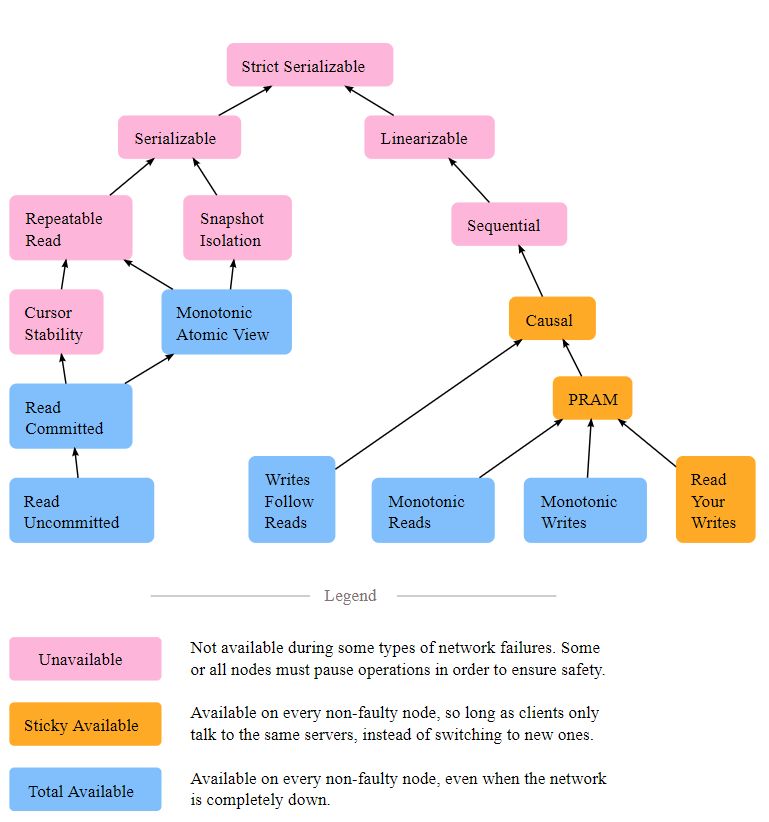
\includegraphics[scale=0.4]{images/consistency models.PNG}
     \caption{Picture from jepsen.io/consistency}
     \label{fig:jepsenioconsistency}
\end{wrapfigure}


For explaining the the concepts within consistency i will use the a paper by Ballis et al on "Highly available transactions"\cite{10.14778/2732232.2732237} that displays a good model for presenting the different consistency models and their relation to other consistency models.\\


\subsection{Strict Serializability}

For a system to be Strict Serializability, it is required that the entire system operationally appear to occur in the order, with regards to both the order and the real time of the operations. within the CAP theorem this would be considers a CA system.\\
\vspace{5mm}

Formally Strict Serializability is define as as Serviceable system that is compatible with a Time dependent order.
"A history is serializable if it is equivalent to one in which transactions appear to execute sequentially, i.e., without interleaving. A (partial) precedence order can be defined on non-overlapping pairs of transactions in the obvious way. A history is strictly serializable if the transactions’ order in the sequential history is compatible with their precedence order."\cite{10.1145/78969.78972}\\
\vspace{5mm}
Here it should be clarified that the obvious way that that if we have transaction A and B, That A proceeds B if A Completes Prior to Transaction B Begins´ or in other worlds a Serializable system with the time constraint from Linearizability.

SS-R cannot be totally or sticky available in the event of a network partition, in this case some or all nodes will be stuck. this is due to the nature of the Strict serializable consistency model, where transaction operates on the system on a whole, as in case of a partition in the distributed system this is impossible. there can be cases where replicate nodes are partitioned from the primary nodes where the primary nodes can continue with some degradation but where the replicas either shutdown or serve stale data. in case of primary nodes partitioning the system would be unable to resume due to not being able to commit a given transaction to the entire system.


\begin{table}[h]
\begin{tabular}{llll}
T1   & T2   & T3   & T4   \\
w(1) &      &      &      \\
r(2) &      &      &      \\
c    &      &      &      \\
     & r(1) &      &      \\
     & r(2) &      &      \\
     & c    &      &      \\
     &      & r(3) &      \\
     &      & w(4) &      \\
     &      & c    &      \\
     &      &      & r(1) \\
     &      &      & c   
\end{tabular}
\caption{Transactions are ordered chronological in time, and executed as such.}

\end{table}

\subsection{Serializable}

Serializability is a relaxation of Strict Serializability consistency model that foregoes that real time constraint, it defines systems where transactions occur in some total order, It is formally defined in the ANSI SQL 1999 spec as follows. "The execution of concurrent SQL-transactions at isolation level SERIALIZABLE is guaranteed to be serializable. A serializable execution is defined to be an execution of the operations of concurrently executing SQL-transactions that produces the same effect as some serial execution of those same SQL-transactions. A serial execution is one in which each SQL-transaction executes to completion before the next SQL-transaction begins."\cite{ansisql1999}\\
\vspace{5mm}

The above implies that Serializability of the transactions does not only apply to the objects in use but the system as a whole, this means that in case of a network partition some or all notes will be stuck until the network is healed. Further as no real time constraint is enforced,  we can observe stale reads, This occurs when Process A completes a Write, Then process B begin a read, the read is not guaranteed to observe the Write from process A, 

There is a further limitation of Serializable due to having no real time constraint, SR is allows pathological orderings. This allows a serializable database to discard write and increment operations that are never observed by executing them at the very end of the history, furthermore read operations can always return a empty state by placing the transaction and the beginning of the history. it should however be noted that most implementation does not take advantage of this.

SR follows closely to S-SR with regards to partition tolerance and availability doing partition, and is therefor considered a CA database.

\begin{table}[h]
\begin{tabular}{llll}
T1   & T2   & T3   & T4   \\
w(1) &      &      &      \\
     & r(1) &      &      \\
     &      &      & r(1) \\
     & w(3) &      &      \\
     &      &      & c    \\
     &      & r(3) &      \\
     & c    &      &      \\
     &      & w(4) &      \\
r(2) &      &      &      \\
c    &      &      &      \\
     &      & c    &      
\end{tabular}
\caption{Transactions are ordered chronological in time, and executed such that the operations occur atomically such that they appear to have been executed in order transaction wise. }
\end{table}

\subsection{Repeatable Read}

Repeatable Read closely resembles the Serializable consistency model, however in RR we allow phantoms. This implies that if T1 read a predicate like "select all from alarms with the newest timestamp", another transaction T2 is able to create, or modify values within the predicate before t1 commits. so if the transaction T1 preforms the read again this predicate might not be stable. 

RR contains the above relaxation, however this relaxation implies more than meets the eye. for example repeatable read doesn't guarantee repeatable reads in the sense that we might consider. this is due to RR not requiring any real time constraint, this allow for a situation where process A performs a write, after process A completes process B performs a read, however this read is not guaranteed to obverse the write from process a. Furthermore as no per process ordering of transactions are require process a can write something and then fail to to observe that write in a subsequent transaction. 

It should also be noted that RR allows for the same pathological ordering of operations as a Serializable database.

\begin{table}[h]
\begin{tabular}{llll}
T1   & T2   & T3   & T4   \\
     &      &      & r(y) \\
     &      &      & c    \\
w(p_1 to y) &      &      &      \\
r(p in y) &      &      &      \\
     &      &      &      \\
     & w(p_2 to y) &      &      \\
     & c    &      &      \\
r(p in y) &      &      &      \\
w(z) &      &      &      \\
c    &      &      &      \\
     &      & r(z) &      \\
     &      & w(x) &      \\
     &      & c    &      
\end{tabular}
\caption{T1 shows a example of a valid transaction with a phantom. and t4 could be placed at the beginning of the history returning the "empty" result. both valid transactions within RR}
\end{table}


\subsection{Cursor Stability}
Cursor stability closely resembles repeatable read. where RR locks the objects until commit, Cursor Stability locks the objects until the cursor moves on or until commit. this allows for different behavoir depending on implementation. but formally defined by which phenomena it allows and which it prohibiteds.
\cite{Adya99weakconsistency}\\
\begin{itemize}
\item G-cursor(x): the directed serialization graph, restricted to a single object x, contains an anti-dependency cycle and at least one write-dependency edge.
\item g1:
\begin{enumerate}
\item G1a (Aborted Reads): A transaction observes an object (perhaps via a predicate) modified by an aborted transaction. Intuitively, transactions have to commit for us to read them.
\itemG 1b (Intermediate Reads): A transaction observes an object (perhaps via a predicate) modified by a transaction which was not that transaction’s final modification of that object. Intuitively, transactions have to finish before we can read them,
\item G1c (Circular Information Flow): the Directed Serialization Graph of transactions contains a directed cylce consisting entirely of dependency edges. Intuitively, if transaction T1 is affected by T2, T2 can’t be affected by T1.
\end{enumerate}
\end{itemize}
Futhermore since cursor stability is strictly stronger than read committed, it also prohibits the ANSI phenomena:
\begin{itemize}
\item P0 (Dirty Write): w1(x) … w2(x)
\item P1 (Dirty Read): w1(x) … r2(x)
\end{itemize}

but allows:
\begin{itemize}
\item P2 (Fuzzy Read): r1(x) … w2(x)
\item P3 (Phantom): r1(P) … w2(y in P)
\end{itemize}


\textcolor{red}{TODO Make Diagram}
\subsection{Snapshot isolation}

Snapshot isolation Behaves differently to any of the systesm, it can be consider more as a try: commit() catch: abort(), we preform our transaction in a independent branch and commit/merge to the database on commit, if there ar any conflicts with a already committed transaction we abort.






\subsection{Read committed}
\textcolor{red}{TODO Make Diagram}
\subsection{Read Uncommitted}
\textcolor{red}{TODO Make Diagram}

\subsection{Monotonic atomic view}
\textcolor{red}{TODO Make Diagram}
\subsection{Linearizable}
\textcolor{red}{TODO Make Diagram}
\subsection{Sequential}
\textcolor{red}{TODO Make Diagram}
\subsection{Casual}
\textcolor{red}{TODO Make Diagram}
\subsection{Writes Follows Reads}
\textcolor{red}{TODO Make Diagram}
\subsection{Monotonic Reads}
\textcolor{red}{TODO Make Diagram}
\subsection{Monotonic Writes}
\textcolor{red}{TODO Make Diagram}
\subsection{Read your writes}
\textcolor{red}{TODO Make Diagram}

Two of the consistency models were already mentioned in the previous section namely Atomic Consistency and Sequential consistency, There exist 2 more within common use, these two are Causal+ Consistency and  Eventual Consistency. They differ in way the consistency is handled by all end up in the same state eventually.





\newpage
\section{Faults, manifestation, and causes}


ANSI/ISO SQL-92 [ANS92] defines the phenomena in English as follows:
\begin{itemize}

\item Dirty Read — Transaction T1 modifies x. Another transaction T2 then reads x before T1 commits or aborts. If T1 then aborts, T2 has read a data item that was never committed and so never really existed.

\item Fuzzy or Non-repeatable Read — Transaction T1 reads x and then T2 modifies or deletes x and commits. If T1 then attempts to reread x, it receives a modified value or discovers that the data item has been deleted.
\item Phantom — Transaction T1 reads a set of data items satisfying some <search condition>. Transaction T2 then creates data items that satisfy T1’s <search condition> and commits. If T1 then repeats its read with the same <search condition>, it gets a set of data items different from the first read.
\end{itemize}


In \cite{Berensonetal} read and write skew are defined that occur due data item constraint violations. the exact definition is below.
\textit{(Data Item Constraint Violation). Suppose C() is a
database constraint between two data items x and y in the
database. Here are two anomalies arising from constraint
violation}

\begin{itemize}
\item 
\item \textit{Read skew Suppose transaction T1 reads x, and then a second transaction T2 updates x and y to new values and commits. If now T1 reads y, it may see an inconsistent state, and therefore produce an inconsistent state as output.
In terms of histories, we have the anomaly:  }
A5A: r1[x]...w2[x]...w2[y]...c2...r1[y]...(c1 or a1)
\item \textit{A5B Write Skew Suppose T1 reads x and y, which are
consistent with C(), and then a T2 reads x and y, writes x,
and commits. Then T1 writes y. If there were a constraint
between x and y, it might be violated. In terms of histories:}
A5B: r1[x]...r2[y]...w1[y]...w2[x]...(c1 and c2 occur)
(Write Skew)
\end{itemize}



\begin{table}[h]
\begin{tabular}{|l|l|l|}
\hline
Phenomenon & Anomaly Interpretation                           & Comment \\\hline
Dirty Read & w1(x) ... r2(x) ... (a1 and c2 in any order)     &         \\\hline
Fuzzy Read/Non-repeatable read & r1(x) ... w2(x) ... c2 ... r1(x) ... c1      &         \\\hline
Phantom    & r1(P) ... w2(y in P) ... c2 ... r1(P) ... c1 &        \\ \hline
\end{tabular}
\caption{r:read, w:write, a:abort, c:commit}
\end{table}


From this knowledge a table can be made that gives us an overview of the isolation levels and what behavior and the trade off they have.
Isolation level	Read phenomena
Dirty read	Non-repeatable read	Phantom read
read uncommitted	yes	yes	yes
read committed	no	yes	yes
repeatable read	no	no	y
serializable	no	no	no


'Dirty read' is when a S1 can read data that S2 has written but not yet committed, It is considered dirty as S2 can rollback the transaction where S1 read data that must be considered non existent. \textcolor{red}{Make example diagram}
\\
The second case of 'Non-repeatable read' is when S1 reads data that is changed by S2 and committed. so if S1 read the some data again they will have changed. this results in two equal select statements returning different results.  \textcolor{red}{Make example diagram}

Phantom read
The Third and last type is phantom read which is a special case of non-repeatable read that occurs when S1 reads data where a where condition is used to specify what data we want. After this initial read, a second session S2 inserts data that meets S1's where condition and commits the data. When S1 issues a select statement with the same where condition, it finds new records. It is called phantom read because the new records seem to be of phantom origin.
 \textcolor{red}{Make example diagram}


\subsection{dirty read}
\subsection{Non-repeatable read and}
\subsection{Phantom read}

\subsection{Long Fork}

\subsection{Split Brain}

The Network is split into 2 or more parts where they each believe different truths,


\subsection{Transient Anomalies}

Process 1 writes A, then process 1 tried to read A but a doesn't exist in the node, and later process a is able to read A

\


\chapter{Database Consistency testing possibly rename to Jepsen}



\section{Introduction}


\section{Modern Database systems, and the trade offs they make.}


Atomicity, and Isolation as we often write the data to a arbitrary node, that accepts after the data has been distributed outside of it's rack, availability zone or region. and where the newest timestamp then overrules all other written data without care of data on other nodes which can breaks Atomicity, and Isolation, as a check and set(CAS), or update statement might uses stale data and due to it's newer timestamp any data written in the meantime gets discarded. Solutions here might require waiting for full distribution of any data prior to the query executing, but this would drastically slow down the entire system. This does however not factor in issues related to system faults
"""

\section{Historically}

Historically this was done with using a manually defined hand coded set of patterns to check how a system behaves with regards to to the isolation levels above, like if some proven invariant hold, or if an anomaly is present in parallel is present by inserting record x and y in two separate transactions and and in two more transactions checking if we can observe x but not y, or y and not x, as this could show how the systems handles long forks and snapshot isolation, and more importantly if it supports it at all.

these checking are generally quite efficient and run in polynomial time, but they only check for a certain patterns and therefor don't give us the larger picture of where issues are present, and only cover a fairly limited set of configurations and isolation levels, and are defined on a system to system basis and no interchangeability is supporter.

This means that this has been a giant scope project where case by case tests are predefined and where we only test for certain scopes, which more importantly mean that tests have been done but the test coverage haven't been perfect and a lot of anomalies are never detected.

\textcolor{red}{Need to add some more to this section, add examples are past test, diagrams, papers etc}

\section{Jepsen}
"
Jepsen is an effort to improve the safety of distributed databases, queues, consensus systems  (...) exploring particular systems’ failure modes. In each analysis we explore whether the system lives up to its documentation’s claims.
"\cite{jepsonio}
\\
\vspace{5mm}

Going from the above quite Jepsen is a way that allows us to check whether a given database system lives up to the requirements and premises that are given, and in a world where distributed, hyper scale or even planetary scale systems are becoming the norm the way data storage is done is required to behave in an expected manner, the reason that expected manner is used rather than correct manner is that we may allow certain faults to occur and eventual consistency to allow for higher throughput applications and that some data may only be required locally as to consider a transaction complete even in the case where some undesirable conditions occur, but these are tolerated to a certain extent. \\
\vspace{5mm}
Two different examples of this is the YouTube 301 views that happened around 2015, where the number of views weren't globally distributed right away. while comments and likes were, this meant two things. \\

Comments were available globally in real time, while views would also commit globally doing low load times, or off hours to maximize utilization of resources.\\
\vspace{5mm}
another more modern scenario where the real time data distribution and correctness is of the utmost importance is within transactions in the finance industry,  where we only want to consider a financial transaction committed once all shards of this data is replicated and the 'old' balance is non longer available, otherwise we could reach a condition where worst case a client is able to draw a negative balance on their account or where one of the transactions isn't recorded as only one of the two transactions is recorded.\\


\section{State of the art.}

The State of the art is Jepsen, or rather one of the State of the Art projects.

Jepsen supports quite a few different modules but the most power full features goes by the name Elle, inferring isolation anomalies from Experimental Observations. \\
\vspace{5mm}
The way this works is be inferring a dependency graph between client side observations and the database version history. This is done by carefully selecting database objects and operations such that the database reads reveals information about the version history.\\
\vspace{5mm}
this means that Elle is able to reveal any anomaly and provide a concise explanation as to why a fault occurred with information of what conditions were present to cause this fault to occur. Using this information we are able to say how a system behaves, what level of isolation and which behavior we'll see as well as what promises the system makes and how does promises are reflected in reality.\\
\vspace{5mm}

And these things can be manifested in multiple ways, some cases are as mentioned earlier in the paper accepted as eventually consistency and performance is valued higher or some applications where loosing some data points are acceptable to allow for higher write throughput.\\
\vspace{5mm}

and the same does for stale, dirty, non-repeatable and phantom reads aren't an issue. this could be on hyper scale social networks where if you see something that was deleted, or if the newest posts, comments and likes aren't distributed across the all notes, but they will eventually. but this is a trade off that is done to allow for much higher write performance as the chance a user is making chancing to the same page on two different nodes/clusters are minimal and the required performance drop required to facilitate the guarantee that all data is always up to date would mean that the system wouldn't scale at the rate it's required, this also brings up another interesting topic, approximate programming, where a program doesn't always have to return the correct output, but if we can see a magnitude speedup of a program and accept a faulty result rate of a few \%, then the cost saving and capacity increase could very much be worth it. this could be in the case of Netflix and amazon recommencing products and services, it doesn't have to be perfect and maybe sometimes the result is wrong but if it means we're able to serve a lot more customers before having to degrade services or maybe having it as a step in the service degradation levels to support as many users as possible. \\
\vspace{5mm}
but a lot of this lay outside the scope of this thesis but it's also a super interesting field that will probably see grow in the next decade.





\section{Past jepsen tests}

https://aphyr.com/posts/294-call-me-maybe-cassandra


https://aphyr.com/posts/291-call-me-maybe-zookeeper



\section{related work to Jepsen}


K. Kingsbury. Knossos.
https://github.com/jepsen-io/knossos, 2013-2019.

G. Lowe. Testing and Verifying Concurrent Objects.
Concurrency and Computation: Practice and
Experience, 29(4), 2017

J. M. Wing and C. Gong. Testing and Verifying
Concurrent Objects. Journal of Parallel and
Distributed Computing, 17(1-2), 1993.

P. B. Gibbons and E. Korach. Testing shared
memories. SIAM Journal on Computing, 26(4), 1997

S. Burckhardt, C. Dern, M. Musuvathi, and R. Tan.
Line-up: A Complete and Automatic Linearizability
Checker. PLDI ’10, 2010.


TODO move these to BIB file and write this section





\newpage
\chapter{Modern Datastores}

\section{Introduction}

The Thesis will primacy focus on Service Fabrics but investigation into other data stores in also done to allow comparisons and investigation into what different models affect the behavior of the database systems.

\section{Service Fabric}
\subsection{Introduction}

Service Fabric (SF) is a presented as a distributed systems platform something akin to Kubernetes (K8S), where the user is able to build, deploy and scale micro services and containers, one of the key points presented by on Azure Service Fabric is that you're able to run stateful services. It's presented by Microsoft as the backbone of their core services and data stores.\\
\vspace{5mm}

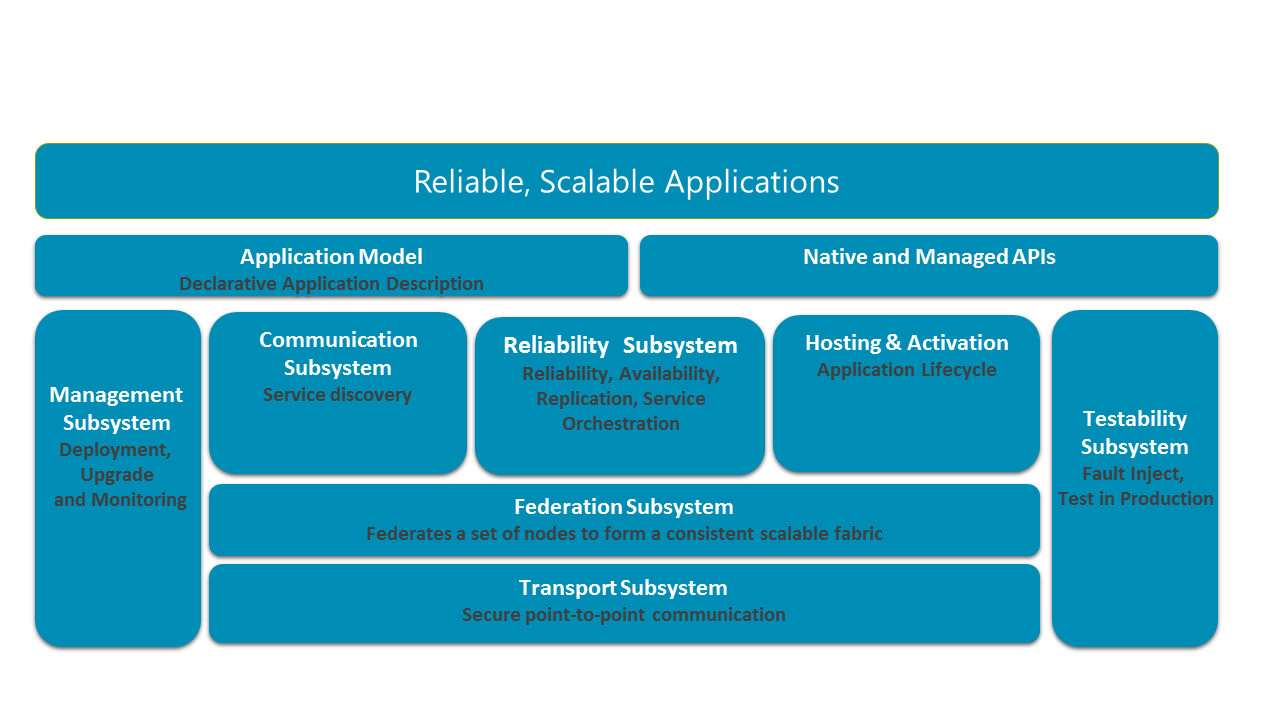
\includegraphics[scale=0.5]{images/service-fabric-architecture.png}

\subsection{System Architecture}

The architecture behind Service Fabric is built via a layered approach, that by Microsoft's words allow developers to write applications that are highly Available, Saleable, manageable and testable. These layers are built on 5 Core and 2 supporting subsystems.  our main interest lies within the reliable collection so i will only be investigating the layers and services that lay below this.\\
\vspace{5mm}



\subsubsection{Transport subsystem}

The lowest layer in the core stack that provides secure communication within the cluster itself and between the cluster and clients. This functionality is provided via point to point communication channels that support one way and request reply patterns, in other terms UDP and TCP. This also provides basis for broadcast and multicast within the cluster. Security is handled via wither windows security or x509 certificates. (TODO these might be serving the name purpose and the documentation might just be odd.)\\
\vspace{5mm}

\subsubsection{Federation subsystem}

The next subsystem in the stack is the Federation subsystem that uses the communication channels provided by the transport subsystem to gather the nodes in the system into a unified service fabric cluster, and provides system primitives that allow for Failure detection, leader Election and consistent routing within the distributed system.\\
\vspace{5mm}

The core of the subsystem is built around a SF-ring that was developed internally at Microsoft in the early 2000s, where both keys and nodes are mapped to a point in the ring, with keys being owned by the node closest to it in the ring. where each node also uses this ring to keep track of its immediate successor and predecessor nodes that it stores in a Neighborhood set, this set is then used by the Federation layer to run consistent membership and failure detection. Nodes also maintain long distance routing partners that are used for consistent routing.\\
\vspace{5mm}

The membership and Failure detection is doing using tow key design principles.\\
\vspace{5mm}

Strongly Consistent membership and Decoupling Failure Detection from Failure Decision\\
\vspace{5mm}

\begin{itemize}
    \item \textbf{Strongly Consistent membership} All nodes must monitoring a given nodes status must agree on weather the node is up or down. for use in the SF ring this means that the all nodes on the node's Neighborhood set must agree on its status.
    \item \textbf{Decoupling Failure Detection from Failure Decision}: failure detection protocols can lead to conflicting states, therefor the decision is decoupled from detection.
\end{itemize}
\vspace{5mm}

To solve the issues of decoupling the failure detection and decision that is used need distribute all decisions to the responsible nodes and ensure that these decisions are all done in a consistent and reliable manner. For the monitoring aspect of this s distributed monitoring and leasing solution is implemented by SF. This implementation solves this via Lease Renewal Request(LR) and LRack. A node is simply required to maintain valid leases from all of it's monitors and these leases have to be renewed every lease period, this leasing period is calculated based on round trip times but is typically around 30 s. If a node fails to renew any of these leases it considers moving itself from the set, and if a monitor misses a request from It it considers marked the monitor as failed. both these decisions need to be approved by a Arbitrator group. if a node fails to receive a LRack within a timeout based on round trip time it repeats the LR until it receives a LRack, Due to the nature of the SF-ring these monitor relations are symmetrical, but this Lease protocol is still run independently, there are however other cases, It a node fails the renewal process is stops renewing leases to any other nodes, or if a node detects a other node as having failed it stops sending renewal request to it. these 2 cases have the potential to cause inconsistencies if they were operating alone, however decision of deciding if a node is down or up is up to the Arbitrator group, which maintains consistent memberships. \\
\vspace{5mm}

The decision of deciding on failures is preformed by the Arbitrator group this is separate from the neighborhood set. They operates independently and have two it has two ways of deciding if a given node has failed. The way that the groups stays consistent when members join or leave the group is that when a Arbitrator joins the set, it initially rejects all requests in the first t seconds, this is done to prevent new Arbitrator making conflicting decisions with the excising nodes, and to prevent failed nodes to exist in the distributed membership protocol. this ensures that detected nodes leave before being forgotten.\\
\vspace{5mm}

\begin{enumerate}
    \item X detects Y as failed and sends fail(Y) to the arbitrator
    \item The arbitrator Ads Y to a recently failed list and sends ack(fail(y)) containing a timeout for Y to X, if The arbitrator already marked X as having failed and ignores the request, 
    \item If X receives this request it waits for the TO to claim Ys area of the ring. and if re receives no response within the timeout it leaves itself.
\end{enumerate}

If a node is already in the recently failed list it returns the same response as the the first reporter except it calculates in time since first detection so the portion of the ring is claimed by the neighbors at the same time. This also means that the routing can continue after to with a laxity added. as all routing request for a node are added to a queued if a node is marked a failed. and the queue is released after TO+laxity that allows a neighboring node to claim that part of the ring and allows to these routing request to be preform when by it's successors.\\
\vspace{5mm}

If the case of two nodes report each other as failed the conflict is resolved either by majority, eg the node that was reported first to the most Arbitrators leave or an alternate variant that heals the membership if both nodes are healthy and allows both to stay. in cases of network congestion or partitions that result in multiple nodes detection each other as failed, in traditional distributed hash tables this can result in inconsistencies in the membership lists or ring. \\
\vspace{5mm}

The implementation in SF is presented as being failure tolerant towards cascade failures as the decision isn't made by the detectors themselves but by arbitrators. an example is used that if a given node is only dependent by it neighbors and ½ of them fails to renew it's lease it will leave itself. No mention here is written about how the node handles being fragmented into two partitions and rejoined later, but mentions that this approach scales to entire data centers, no mentioned about how it scales across regions or outside of data centers.\\
\vspace{5mm}

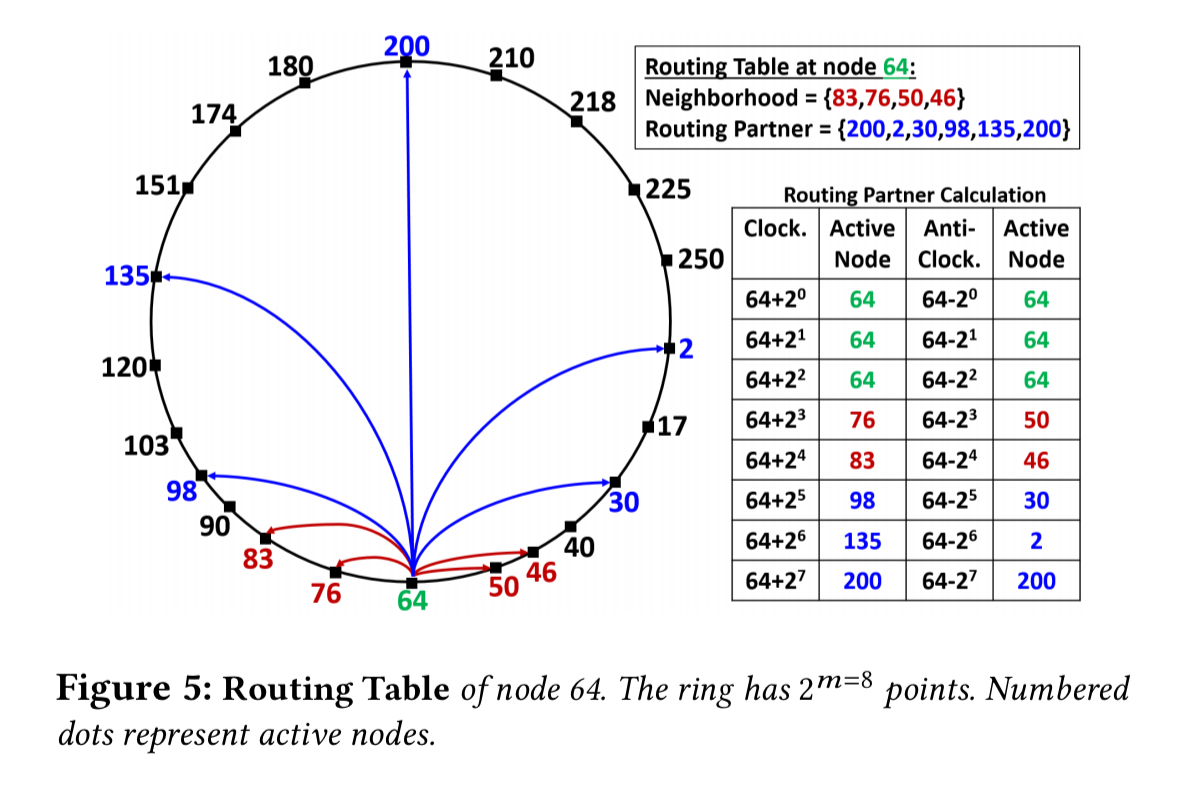
\includegraphics[scale=0.3]{images/servicefabric-fig-ring-topology.jpeg}

SF-Ring and consistent routing.(need to rewrite/reword this to a more coherent sentence.)

The Distributed Hash table used for service fabric routing is a evolution of SF-ring that was developed within Microsoft in the 2000s. The routing used offer symmetry and due to this it allows bidirectional routing that allow for lookup and routing via binary search, this allows SF to in practice routes message around the ring in a fast manner, with multiple routing options in that there always exists 2 routing partners on either side of the destination that both helps distributed the load and is able to route even with stale routing tables. Initially all packages were routed using this method however this has changed over the years, today the hash table is used to build a routing table and maintain it when a new node is added to the cluster, and ti route message to virtual addresses. After discovery a direct route is used via the destination IP address. \\
\vspace{5mm}

Routing tables work differently depending on the size of the cluster. however it is able to route in two ways, If the size of the routing table is smaller then the number of nodes a direct route is used, if there exist more nodes in the cluster then the routing tables it stitches to routing via routing tables to reduce memory consummation but causing an increase in time complexity to O(Log(n)) from O(1)\\
\vspace{5mm}

Routing Tokens.
Each node owns a token that includes a portion of the routing token it is responsible for. The sf-ring protocol ensures two properties, That each token is only owned by one node at any given time, and that eventually every token is owned by 1 node. This is ensure in the way that SF handles nodes joining and leaving the ring. Initially the bootstrap node owns the entire ring. after this inertial bootstrap node any joining node will split the ring segment between them.(TODO I was unable to find information on this precisely is handled however from the wording in the paper the initially split would be 50/50 and a third node would be 50/25/25?  is it split evening it 33/33/33 but a Fourth node would be 22/22/22/33 that would cause unbalance unless some shifting is done)\\
\vspace{5mm}


These routing tokens are also used for leader election, Simply the owner of a given key is the owner.

\subsubsection{Reliability subsystem}
The reliability subsystem is in charge of load balancing, replication and availability. These three aspects are provided via 3 services, Failover Manager, Naming and Resolution, and a Placement and Load Balancer service.\\
\vspace{5mm}

The Failover Manager is running as stateful service, that has a instance running on each node in the cluster, that provide 3 actions, start a replica, move a replica, reconfiguration.\\
\vspace{5mm}

\begin{itemize}
\item \textbf{Create a replica} Create a new replica when instructed by the PLB
\item \textbf{Move a replica} migrate a replica when instructed by the PLB to a different node.
    \item \textbf{Reconfiguration} If a primary replica becomes unavailable to promotes a secondary as the new primary, in case the old primary comes back only it is demoted to secondary. 
\end{itemize}

A service called Failover Master Manager is also running that is able to restart the failure manager via a cached state in case it fails. in case the master fails it is able to rebuilt its state via the SF-ring, the Master Failover manager is running on the node who's token range contains ID0.\\
\vspace{5mm}

The naming and resolution service maps instance names to endpoints that running services are listening on, this also allows for consistent routing from outside of the cluster via URI that doesn't change over a their lifetimes.\\
\vspace{5mm} 

The Placement and Load Balancer(PLB) service is stateful and is in charge of placing replicas and instances of services at nodes and ensure even load throughout the cluster. they claim that unlike other solutions where services are hashed onto the ring in SF the PLB explicitly assigns each services replicas Primary and Secondaries to nodes in the Ring. it continually monitors the cluster for available resources to both assigned and migrate services to underutilized nodes and migrates services away from a node that is about to be upgraded or is overloaded due to a long workload spike.\\
\vspace{5mm}

The technique used for selecting placement of nodes is done via Simulated Annealing, as it is presented to provide a near optimal solution as to where services can be placed, This way the system is modeled is via resource use in the system where a even load is desired, but some constraints need be met such as fault tolerance, avoiding replica co location and some service might have strict set of nodes to run on. \\
\vspace{5mm}


\subsubsection{Reliable Collections}

Reliable collections provide stateful services in Service fabric via Reliable Directories and reliable Queues that are available for C\# and java programming, and are promised to be:
\begin{itemize}
    \item Available and Fault-tolerant via replication,
    \item Persistent via disk
    \item Efficient via asynchronous via API that are non blocking. 
    \item Transnational via APIs with ACID semantics.
\end{itemize}

One of the key differences between storage systems build on SF and other highly-available systems is that states are kept locally in the replica while also being made highly-available, this causes most reads to be local.\\
\vspace{5mm}

Writes are relayed from the primary replica to secondary replicas via passive replication and are considered complete when the majority of secondaries acknowledges it. the relaxations allow an application to achieve weaker consistency by relaxing where a read can go, eg always read from primary to read from secondary. \\
\vspace{5mm}

SF is presented as the only "self-sufficient microservice system that can be used to build a transactional consistent database which is reliable,available, self-*, and upgradable because the lower layers assure consistency"\cite{SFpaper} \\
\vspace{5mm}

\paragraph{Consistency models/isolation levels}
SF reliable collections promise two Select-able consistency models that the user can pick. Repeatable Read and Snapshot isolation. eg there is no promise about Serializability of the transactions.\\
\vspace{5mm}

\begin{table}[h]
    \centering
    \begin{tabular}{l|l|l}
     & \multicolumn{2}{c@{}}{\text{Role}}\\
    \text{Operation} & Primary & Secondary \\
        Single Entity Read & Repeatable Read & Snapshot\\
        Enumeration, Count & Snapshot & Snapshot
    \end{tabular}
    \caption{isolation level defaults for Reliable Dictionary and Queue operations.}
    \cite{SF_RC_Transactions}
\end{table}

\section{Programming for Service Fabric}


\section{Comparison}

In many of the papers published by Microsoft a lot of comparisons are made to Cassadra, Redis and Redis Therefor comparisons will be made to these as they are compared in a lot of aspect, the investigation won't be as deep as with SF but investigation of consistency and failure modes will be be done.

\subsection{Cassadra}

\subsection{Redis}

\subsection{Dynamo}


\chapter{Jepsen Test on Service Fabric Reliable collections}

\section{Introduction}

The Goal of the thesis was to attempt to preform a Jepsen test on service fabric with it's reliable collection as the data store feature that powers a lot of the services being the target of this endeavor. To preform such a test we need to build up both a testing suite, APIs and libraries to allow for a connection between the Jepsen service and the Service fabric core components. there for a few different applications and services need to be learnt, understood, designed, implemented, test, executed, and at last the data generated from this can be analyzed.
\begin{itemize}
    \item Learning the required tools to implement the services and applications in the first place. C\#, Clojure, and Service Fabric itself as well as reliable collections and lastly Jepsen itself
    \item Understanding the problem, requirement, topology, architectures and how we want to test these things
    \item Designing the Services, Libraries, APIs, testing suite, and the infrastructure and networking of the cluster and azure.
    \item implement the  Services, Libraries, APIs and testing suite required for things to talk to each other.
    \item Test all the code and configurations and ensure things work as intended.
    \item execute the test itself
    \item analyse the data from the test.
\end{itemize}

I will only write deeper about designing, implementing testing, executing and analysing the results. however this does not mean that the learning and understanding phase of the project was any smaller, quite the contrary, Learning 2 new programming languages that I've never interacted with before isn't a easy task, adding in the complexity of write code for cloud framework that i had no prior experience working on didn't help either. spicing it with up with outdated documentation, incompatibility between versions of the framework and lack of debugging tools and broken tools meant that a lot was done via eyes blind brute forcing solutions to a lot of issues due to lacking features on the Linux version of the cluster.\\

\section{Design \& implementation}
The Design of the services required for preforming the Jepsen test were designed on the fly as no prior experience was had with Service Fabric, Jepsen, C\# or Clojure.
\subsection{Initial Design}

The initial design of the of the testing suite contained two applications, A stateful service Fabric application and a Clojure application running the Jepsen test.

\subsubsection{Service Fabric Stateful Service}

The Service Fabric stateful service should contain the desired operation that our Jepsen test can interact with, the first designed endpoints were insert/add, Update, Check and set, delete and delete all on a reliable directory class.It would be implemented using C\# as the lack of documentation for java made this this seem easier in the beginning and due to all documentation being in C\#. The service would expose these end point via a web endpoint and kestrel was selected for this as it was a native provided already integrated into SF and was the one most ex samples used and was therefor deemed the safest choice to proceed with.\\
\vspace{5mm}
A diagram of the service looks as the following. \\
\vspace{5mm}
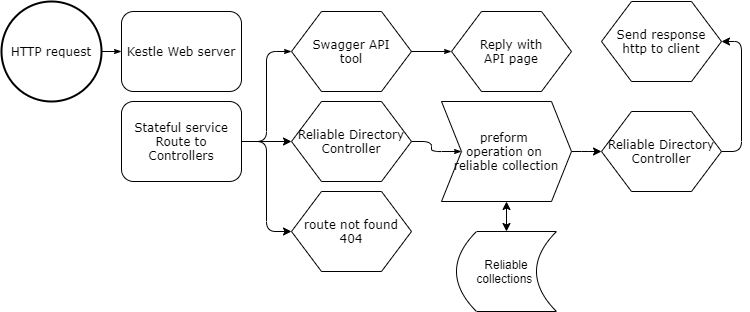
\includegraphics[scale=0.5]{images/Design_Stateful_service_1.0.drawio.png}

This implementation contains 2 main codebases. The c\# dotnet web service that acts as a restAPI to the reliable collections using 3 controllers for the 2 default data structures implemented in the framework, and a Clojure codebase that contains the test suite as well as the API connector that handles parsing, connections and connections faults.

\subsubsection{Infrastructure}
The infrastructure in centered around v-net containing 6 Virtual machines all running linux, in this case ubuntu 18.04 and 20.04 for the jepsen host, I'll refer to the service fabric nodes from n1-n5 and the jepsen host as jepsenhost from now on.
The 5 service fabric nodes are mostly self managing, applications can be deployed via either the Azure Service Fabric CLI\cite{https://docs.microsoft.com/en-us/azure/service-fabric/service-fabric-cli} or via visual studio\cite{https://docs.microsoft.com/en-us/azure/service-fabric/service-fabric-tutorial-deploy-app-to-party-cluster} which was the process used doing the development stages of the project.

This Jepsenhost was management via ssh and rsync to deploy the newest version of the test code. Here a deployment pipeline could have been used to handle all of this by fetching, building and deploying via Jenkins or such a service but due to the goal of the project not being automated testing of Service Fabric, a bashcript instead used that deployed code, started applications, ran the test and retrieve results was used instead. rsync was used instead of scp to reduce the files being move back and Fourth from the deployment machine and the test cluster. 

The topology of the network is so that
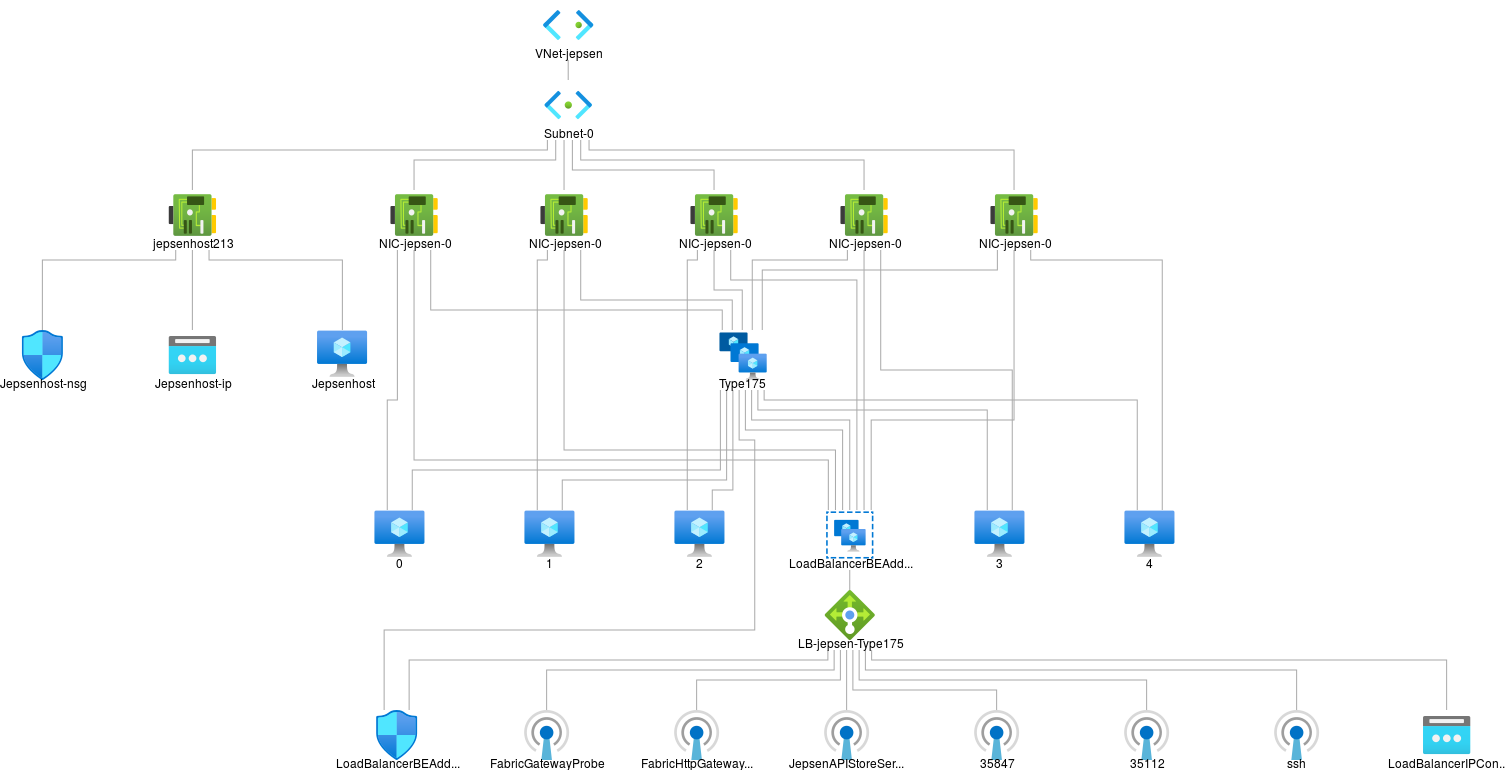
\includegraphics{images/topology.png}

All traffic resides within the cluster and the load Balancer is only there for testing of the application and check if all endpoints work as expected.

\paragraph*{Node Sizes}

The initial node sizes were 2 cpu cores and 8 gbs of ram along with 20 gb local storage, as this was thought be enough to handle the workload of the test. This was later revised as the nodes had issues with disk space and often took a long time to setup and get ready for any given deployment, this was resolved by upgrading the size of the nodes to 4vcpu, 16gb ram and 80gb local storage per node. This configuration resulted in a much more well-behaved cluster. and this node size was kept for the reminder of the test. However the jepsenhost is slightly underdimensioned compared to the workload it handles when computing on the result of the test. This is primary due to OOM errors that could be resolve with wither lowering the search space of the test or increasing the memory of the node itself.

\section{Services}
as mentioned earlier running these tests required multiple components, The stateful service that hosts the reliable collections from SF Reliability subsystem, a restless front-end that provides this data to clients via RESTAPI, a driver that handles the connection to this api and finally the Jepsen test suite itself consisting of both test suite and checker of the transactions and fault induced of the end system.

\subsection{SF services}
Using the 2 services approach as recommended from Microsoft provides multiple benefits but also a few negatives. the prime benefit it abstracting from the backend and adding a layer of validation, routing, and protection of the backend service. as well as greatly reducing the time that connections are held open to due RR times as all connections to the data store is kept within the cluster. 
\subsubsection{Stateful Reliable collection service}

The stateful services provides 3 separate controllers that each provides one of the built in reliable collection types provided by service fabric. Reliable dictionary, reliable queue, and reliable concurrent queue. Fault handling is also handled at this stage where any fault stemming from the transactional issues is returned to the client via http status codes\cite{https://en.wikipedia.org/wiki/List_of_HTTP_status_codes}. eg node not primary, accepted, result not found.. etc. 

The fronted service simply provides these same apis but with wrappers and routing in case of a portioned design. This layer could also be used to built additional features but this was not the case as only the bare transactions supported by the reliable collections layer was needed.

\subsection{Jepsen test suite}
The Jepsen test suite contains many layers and two main components a connector that connects to the service fabric services, and the test suite itself.

The drive is the simplest service that is based on a raft api that was completely rewritten to interact with the SF API along with a custom fault handler that is able to parse both the result that the reliable collections api provides along with with the http codes in case something doesn't behave as intended.

The Jepsen test component contains 6 classes. a runner, a db class that prepares for the test, a client that interacts with the driver, nemesis that induces faults in the cluster and 3 workloads, queue, cqueue, and dict. testing the 3 separate types provided by service fabric.

The runner type is the main class that handles defaults, cli input and test selection along with code that handles common behavior between the test. nemesis, db, along with other features that are mutual for all services that run in service fabric.

the db class that is in charge for spinning up and tearing down the services along with functions for stating and stopping workers in the cluster.

the nemesis class that contains the functions that kill, partition or otherwise mess and attempt to break the cluster.

the 3 workloads.

These each contain client for the test defining what endpoint to reach out to, a generator generating a sequence of transactions to preform on te database, and a checker that checks if our data stored behaved as expected.

all types are expected to follow the repeatable-read consistently model. where the concurrent queue does best effort to meet the FIFO order of queued items compared the the normal queue following a FIFO ordering.



\subsection{Implementation of the initial design.}

The initial designed first targeted the reliable collection dict datatype. and presented a few issues with the design and implementation details that was not considered. 

The biggest hurdle here was developing code for the service fabric Linux cluster due to a non feature parity between it and the windows cluster which caused non favorable conditions such as no debugging, binary dump files that weren't readable by any tool available. 

Here a great amount of time was spent debugging, changing configuration files, stripping any unneeded libraries and rolling back to older versions of frameworks. it should be noted that the service fabric framework was kept at the newest release while .NET and similar aspects where rolled back to older releases.

All of these attempts were however frugal, after spending newly 2 months deleting all code, starting from scratch using a different skeleton code. trying the implementations via java, going back to C\# getting a working solution on the windows service fabric implementation i reached out to Mikkel from Microsoft. 

The issue turned out to be 2 fold.
\begin{itemize}
\item .NET needing to be rolled back to 3.5
\item the entry point having to be defined via .NET and the name of the DLL file. this was something i attempt prior by using a entry point.sh that did the same while his solution was just replacing where the windows version has .exe with .DLL and as a .NET entry point.
\end{itemize}

Finally i had a runnable version on Linux, or rather. i had a way to run my application on Linux as the issues didn't stop here. the Feature parity was still there. the dns service was still missing, this required a lot of endpoints to be hard coded, which induced as one active replica of a given service per node. eg we can only have 1 service running per node which would greatly reduce horizontal scaling of the partitions which would greatly increase the number of partitions required to handling greater workloads. running larger partitions on each node is also an option but from a performance, availability, and reliability it's much effect having lots of smaller nodes instead of one large database instance that require a lot of broadcasting to each partition replica.



This required some changes to the design but was resolved by removing of the layers in the application and accessing the stateful service directly, or rather creating a parallel service in case the other services were required later.

\subsection{2nd iteration of the design.}

This 3rd service should simply provide the API directly from the stateful service, as the transactions are going to behave the same on a single partition as with 500 partitions. this 3rd service was configured such that replicas were active. this implies two things: Routing is no longer an issue, we need to route primary traffic to the primary node from our Clojure connector.

this issue can be resolved in two ways. one is rather quick, while the other queries the SF cluster for which node is primary. the quick solution of just defining the primary at launch and from there checking which node allows writes in case the current node start blocking writes. this is a messy solution but as it doesn't induce noise in the data as these transactions are simply rejected/discarded it is therefor not an issue. optimally we should query the SF cluster for primary node, this implementation could chosen but as it takes more time and doesn't yield any further results this is deemed unnessesray.

\subsection{Implementation of this design}


The implemnetation of this interated design was supposed to have been been fairly streight forward however the non feature parity again poked it ungly head out again. The issues that arrived from here was mainly due to a change in the settings of the service fabric version which chaused some warnings to turn into errors. that exposed my inexperiance of working with the dotnet framework and the service fabric API. this issues were however eventually ironed out but a lot of times was lost due to the lack of debugging output from the cluster which turned the development cycle upside down as i had no way to execute the code without service fabric but the code wouldn't un on service fabric. The issue here ended up beging related to some changes in allowed port ranges that were allocatable to services and therefor killed the application as it was using an illigal port. these warnings were however not displayed correctly in the linux distribution.

After this step the services to ready to test, as mentioned earlier in the paper 6 nodes are used to preform the test. 5 cluster member nodes and 1 jepsen test node. 

The steps to deploy and run the tests is as follows.

\begin{enumerate}
\item Deploy Cluster via a vm scaleset with a SF image, the jepsen host, a proximity group to prevent network issues, setup vlan and add the 6 servers, add a public IP to sasilirate connections to the test envoriment, Configure storage devices and firewalls to prevent undesired access and noise in the testing.
\item Deploy the SF applications
\item connent to the Jepsenhost server and sync test framework.
\item run test framework with desired perameters
\item pull test result to local machine to analyse results.
\end{enumerate}

For the first few rounds of testing everything went alright, however after running a few test exsamples 


\subsection{Issues}


Linux and windows versions being far from interchangeable and applications and services that function on windows/local machines fail crash on deployed cluster

visual studio being unable to load .dmp files to debug crashed applications from the cloud.

Visual studio remote debugger not working

\subsubsection{Azure}

Configuration issues,

Cluster becoming unhealthy/corrupt and nodes not being configured correctly after a reimage.


\subsection{Jepsen Service}


\section{Execution of the test}

Steps.

1 start Service Fabric cluster in azure.
2. Add Jepsen node to Vlan of the cluster.
3. Deploy SF application to the cluster. This is currently done via Visual studio but could also be automated from the jepson node.
4. Deploy Jepsen code to the Jepsen node.
5. Run Jepsen test.
6. Retrive Test data from test node.
7. Clean up.


\section{Results}




%\blinddocument

\chapter{Related Work}

\chapter{Conclusion and Outlook}
\section*{Conclusion}

\section*{Outlook}


\section{Future Work}
 Atomic clocks ?    




\newpage
\chapter{Appendix}

\pagestyle{empty}
\printbibliography

\section{Proposal}
\section{'Jepsen methods usage for ACID compliance in Hyperscale Cloud Frameworks'}

\section{Introduction}
The goal of this project is to assess how Jepsen\footnote[1]{https://aphyr.com/tags/jepsen } tests allow us to verify the properties of ACID\footnote[2]{Database Management Systems by Raghu Ramakrishnan \& Johannes Gehrke  ISBN13 9780071231510} in a cloud system.
The Jepsen test is a method used to evaluate the compliance of a system in relation to the ACID properties. This is done is by analysing the system via Blackbox\footnote[3]{https://youtu.be/tRc0O9VgzB0?t=293} tests , in the sense that the internals of the system work are not relevant. We look at the service from a client-side and not any underlying structures or frameworks.
The ACID properties are 
\begin{itemize}
\item	Atomicity \\
Guarantees that each transaction is treated as a single "unit", which either succeeds completely or fails completely 
\item	Consistency \\
Ensures that a transaction can only bring the database from one valid state to another
\item	Isolation \\
Ensures that concurrent execution of transactions leaves the database in the same state that would have been obtained if the transactions were executed sequentially 
\item	Durability \\
Guarantees that once a transaction has been committed, it will remain committed even in the case of a system failure 
\end{itemize}
\footnote[2]{Database Management Systems by Raghu Ramakrishnan \& Johannes Gehrke  ISBN13 9780071231510} \\
We plan to apply these methods on Service Fabric\footnote[4]{https://docs.microsoft.com/en-us/azure/service-fabric/service-fabric-overview  } , to verify if this system is compliant with the ACID properties. Service Fabric is a framework developed by Microsoft, designed to allow developers to build Hyper-Scale Cloud (HSC) deployments on the Azure\footnote[5]{https://microsoft.com/en-us/azure/ } platform.
The motivation behind this thesis is to study the ACID properties in an HSC environment and evaluate how the constraints of ACID hold up in practice, as well as verifying if these constraints are met, and more importantly if they are not. 
\section{Plan}
     
The project is segmented into three parts. The writing of the report will take place at all times throughout the process, and the final phase should be a finalization and corrections phase.  
\subsection{The study phase  }
\begin{itemize}
\item	The first part of the study will focus on analysing the previous\footnote[6]{https://jepsen.io/analyses } Jepsen tests performed on other systems. This will allow us to define a strategy in terms of: which tools, tactics and methods are worth investigating, and what type of faults should be taken note of. This information is useful for two aspects:
\begin{itemize}
\item	where our focus should be when testing,  
\item	which tools and packages we should be familiarize with. 
\end{itemize}
\item	 The second part of the study will centre around “Service Fabric” and getting to know how the framework is coupled together, what vectors we can access the system from, and how we can manipulate the framework to induce fault conditions.   
\end{itemize}
\subsection{The experimentation phase}
\begin{itemize}
\item	In the experimentation phase, we will design and perform tests on the system. If any faults occur, we will attempt to locate where, and why they occur. If the scope and the timeline of the project allow, we will assess whether we prevent the faults from occurring in the future.
\item	The Experimentation phase of the project will include the steps described below. 
\begin{itemize}
\item	Planning of the test, selection of the aspects of the system to be tested, consulting with developers and users of the system to determine if and where undesired behaviour may occur.
\item	Designing the tests and setting up the tools to facilitate those tests.
\item	Writing the tests, verifying they work as intended and setting up a data collection framework to collect the data in a manner that allows our analysis.
\item	Performing the tests on the system in different scenarios, normal conditions and different levels of faults and disaster recovery.
\item	Analysing the data for faults, errors and inconsistencies.
\item	Consulting with DEVs to determine where the faults occurred, and which failures or bugs led to these fault conditions.
\item	Concluding whether “Service Fabric” is ACID-compliant. 
\end{itemize}
\end{itemize}
\subsection{The report phase }
\begin{itemize}
\item The final phase of the project aims at finishing an initial draft, reviewing and correcting it, and finalizing the report for hand-in.
\item	Deliverables 
\begin{itemize}
\item	At the end of the project, there should be a report, the tests and the results from those tests. 
\item	The report written in English and following the standard academic writing conventions will include 
\begin{itemize}
\item	A study on Jepsen tests, describing what they are, as well as why and how they are done.
\item	An experiment in which we will analyse “Service Fabric”	
\item	A discussion on the conclusiveness of the test and the compliance of the framework with service fabric.
\end{itemize}
\item	The code \& data will include
\begin{itemize}
\item	Scripts and code for tests and for analysing the data.
\item	Relevant results and data from the tests. 
\end{itemize}
\end{itemize}
\end{itemize}

\section{Goal}
The goal of the project is to deep dive into Jepsen tests with a focus on “Service Fabric” as the subject. The optimal goal of the project is to verify if the database aspects of “Service Fabric” comply with the ACID properties, and to locate the fault cases in case they don’t.    
Risk assessment 
There are a few risks in the project. In the case no faults are found within the Service Fabric, this reduces the scope of the project. If no faults are found, time allowing, different framework can be analysed. On the contrary, if the number of faults in the framework is more extensive than expected, then the scope of the project may grow uncontrollably. In this case, choices will be made to select a subset of the data to focus on.

\section{Schedule}

% Please add the following required packages to your document preamble:
% \usepackage{multirow}
% \usepackage[table,xcdraw]{xcolor}
% If you use beamer only pass "xcolor=table" option, i.e. \documentclass[xcolor=table]{beamer}

\begin{tabular}{clll}
\multicolumn{2}{l}{Mark Jervelund thesis plan} &                                           &                  \\
                                & Week 45      &                                             &                                                                                                                            \\
                                & Week 46      &                                             & \multirow{-2}{*}{\text{Study Jensen test}}                                                                                        \\
                                & Week 47      &                                             &                                                                                                                            \\
\multirow{-4}{*}{November}      & Week 48      &                                             & \multirow{-2}{*}{\text{Finish study on Jepsen test}}                                                                              \\
                                & Week 49      &                                             &                                                                                                                            \\
                                & Week 50      &                                             & \multirow{-2}{*}{\text{Study Service Fabric} }                                                                                    \\
                                & Week 51      &                                             &                                                                            \\
                                & Week 52      &                                             & \multirow{-2}{*}{\text{Christmas break}}                                            \\
\multirow{-5}{*}{December}      & Week 53      &                                             &                                                                                                                            \\
                                & week 01      &  \multirow{-10}{*}{\text{Structured study 8 weeks}} & \multirow{-2}{*}{\text{Finish Study Service Fabric} }                                                                             \\
                                & Week 02      &                                             &                                                                                                                            \\
                                & Week 03      &                                             & \multirow{-2}{*}{\text{designing the experiment}}                                                                                 \\
\multirow{-4}{*}{January}       & Week 04      &                                             &                                                                                                                            \\
                                & Week 05      &                                             & \multirow{-2}{*}{\text{designing the experiment} }                                                                                \\
                                & Week 06      &                                             &                                                                                                                            \\
                                & Week 07      &                                             & \multirow{-2}{*}{\text{Execute the experiment}  }                                                                                 \\
\multirow{-4}{*}{February}      & Week 08      &                                             &                                                                                                                            \\
                                & Week 09      &                                             & \multirow{-2}{*}{\text{Analyse the experiment}}                                                                                   \\
                                & Week 10      &                                             &                                                                                                                            \\
                                & Week 11      &  \multirow{-10}{*}{\text{Experiment 10 weeks}}     & \multirow{-2}{*}{\text{discover what the findings from the experiment is}}                                                         \\
                                & Week 12      &                                             &                                                                                                                            \\
\multirow{-5}{*}{March}         & Week 13      &                                             & \multirow{-2}{*}{\text{Running additional experiments if needed  Full on write mode}} \\
                                & Week 14      &                                             &                                                                                                                            \\
                                & Week 15      &                                             & \multirow{-2}{*}{\text{Full on write mode} }                                                                                      \\
                                & Week 16      &                                             &                                                                                                                            \\
\multirow{-4}{*}{April}         & Week 17      &                                             & \multirow{-2}{*}{\text{Full on write mode} }                                                                                      \\
                                & Week 18      &                                             &                                                                                                                            \\
                                & Week 19      &                                             & \multirow{-2}{*}{\text{Full on write mode    Send out thesis for feedback}}             \\
                                & Week 20      &                                             &                                                                                                                            \\
                                & Week 21      & \multirow{-10}{*}{\text{Thesis writing  10 weeks}} & \multirow{-2}{*}{\text{Correction} }                                                                                              \\
\multirow{-5}{*}{May}           & Week 22      &                                             &                                                                                                                            \\
                                & Week 23      & \multirow{-2}{*}{\text{goal}}                      & \multirow{-2}{*}{\text{Hand in}}                                                                                                  \\
                                & Week 24      & \multicolumn{1}{l}{}                        & \multicolumn{1}{l}{}                                                                                                       \\
                                & Week 25      &  \multicolumn{1}{l}{}                       & \multicolumn{1}{l}{}                                                                                                       \\
                                & Week 26      &  \multicolumn{1}{l}{}                       & \multicolumn{1}{l}{}                                                                                                       \\
\multirow{-5}{*}{June}          & Week 27      & \multicolumn{1}{l}{}                        & \multicolumn{1}{l}{}                                                                                                       \\
\multicolumn{1}{l}{}            & Week 28      & \multicolumn{1}{l}{}                        & \multicolumn{1}{l}{}                                                                                                       \\
\multicolumn{1}{l}{}            & Week 29      & \multicolumn{1}{l}{}                        & \multicolumn{1}{l}{}                                                                                                       \\
\multicolumn{1}{l}{}            & Week 30      & \multicolumn{1}{l}{}                        & \multicolumn{1}{l}{}                                                                                                       \\
\multicolumn{1}{l}{}            & Week 31      & \multicolumn{1}{l}{}                        & \multicolumn{1}{l}{}
\end{tabular}




%% !TeX root = main-english.tex
% !TeX spellcheck = en-US
% !TeX encoding = utf8
% -*- coding:utf-8 mod:LaTeX -*-

%This smart spell only works if no changes have been made to the chapter 
%using the options proposed in preambel/chapterheads.tex.
\setchapterpreamble[u]{%
  \dictum[Albert Einstein]{We cannot solve our problems with the same level of thinking that created them}
}
\chapter{LaTeX Hints}
\label{chap:latexhints}

One sentence per line.
This rule is important for the usage of version control systems.
A new line is generated with a blank line.
As you would do in Word:
New paragraphs are generated by pressing enter.
In LaTeX, this does not lead to a new paragraph as LaTeX joins subsequent lines.
In case you want a new paragraph, just press enter twice (!).
This leads to an empty line.
In word, there is the functionality to press shift and enter.
This leads to a hard line break.
The text starts at the beginning of a new line.
In LaTeX, you can do that by using two backslashes (\textbackslash\textbackslash).
This is rarely used.

Please do \textit{not} use two backslahes for new paragraphs.
For instance, this sentence belongs to the same paragraph, whereas the last one started a new one.
A long motivation for that is provided at \url{http://loopspace.mathforge.org/HowDidIDoThat/TeX/VCS/#section.3}.

One can write \emph{emphasized text (rendered in italics)} and \textbf{bold text}.

\section{File Encoding and Support of Umlauts}
\label{sec:firstsectioninlatexhints}
The template offers foll UTF-8 support.
All recent editors should not have issues with that.

\section{Citations}


References are set by means of \texttt{\textbackslash cite[key]}.

\begin{filecontents*}{\democodefile}
Example: \cite{WSPA} or by author input: \citet{WSPA}.
\end{filecontents*}
\PrintDemo{style=parallel}

The following sentence demonstrates
\begin{inparaenum}[1.]
  \item the capitalization of author names at the beginning of the sentence,
  \item the correct citation using author names and the reference,
  \item that the author names are a hyperlink to the bibliography and that
  \item the bibliography contains the name prefix \qq{van der} of \qq{Wil M.\,P.\ van der Aalst}.
\end{inparaenum}

\begin{filecontents*}{\democodefile}
\Citet{RVvdA2016} present a study on the effectiveness of workflow management systems.
\end{filecontents*}
\PrintDemo{style=parallel}

The following sentence demonstrates that you can overwrite the text part of the generated label using \texttt{label} in a bibliopgrahie"=entry, but the year and the uniqueness is still generated by biber.

\begin{filecontents*}{\democodefile}
The workflow engine Apache ODE \cite{ApacheODE} executes \BPEL processes reliably.
\end{filecontents*}
\PrintDemo{style=parallel}

\begin{filecontents*}{\democodefile}
Words are best enclosed using \texttt{\textbackslash qq\{..\}}, then the correct quotes are used.
\end{filecontents*}
\PrintDemo{style=parallel}

When creating the Bibtex file it is recommended to make sure that the DOI is listed.

\section{Formulas and Equations}
\label{sec:mf}

\begin{filecontents*}{\democodefile}
Equations $f(x)=x$ inside the text can be provided.
\end{filecontents*}
\PrintDemo{style=parallel}

A list with all available mathematical symbols is provided at \url{http://texdoc.net/pkg/symbols-a4}.

\begin{filecontents*}{\democodefile}
As example the set of natural numbers is given by $\mathbb{N}$.
\end{filecontents*}
\PrintDemo{style=parallel}

For the documentation of editing mathematical formulas read the package documentation of \texttt{amsmath}\footnote{\url{http://texdoc.net/pkg/amsmath}}.

Equation~\ref{eq:test} is numbered and can be referenced in the text:
\begin{filecontents*}{\democodefile}
\begin{align}
  \label{eq:test}
  x = y
\end{align}
\end{filecontents*}
\PrintDemo{style=parallel}

Following equation is not numbered because of using \texttt{\textbackslash align*} as environment.
\begin{filecontents*}{\democodefile}
\begin{align*}
  x = y
\end{align*}
\end{filecontents*}
\PrintDemo{style=parallel}

The template offers \verb+\abs+ to enable the bars scaling well at the absolute value:

\begin{filecontents*}{\democodefile}
$\abs{X}$.
\end{filecontents*}
\PrintDemo{style=parallel}

More details about mathematical environments provides the documentation available at \url{http://www.ctan.org/tex-archive/help/Catalogue/entries/voss-mathmode.html}.


%%%%%%%%%%%%%%%%%%%%%%%%%%%%%%%%%%%%%%%%%%%%%%%%%%%%%%%%%%%%%%%%%%%%%%%%%%%%%%
\section{Sourcecode}
%%%%%%%%%%%%%%%%%%%%%%%%%%%%%%%%%%%%%%%%%%%%%%%%%%%%%%%%%%%%%%%%%%%%%%%%%%%%%%
\Cref{lst:ListingANDlstlisting} shows how to emmbed source code.
With \texttt{\textbackslash lstinputlisting} the source code can be loaded directly from files.

%Listing-Umgebung wurde durch \newfloat{Listing} definiert
\begin{Listing}
  \begin{lstlisting}
<listing name="second sample">
  <content>not interesting</content>
</listing>
\end{lstlisting}
  \caption{The code is separated by two horizontal lines in the listings environment.}
  \label{lst:ListingANDlstlisting}
\end{Listing}

\begin{filecontents*}{\democodefile}
Source code is also available in the text \lstinline|<listing />|.
\end{filecontents*}
\PrintDemo{style=parallel}


%%%%%%%%%%%%%%%%%%%%%%%%%%%%%%%%%%%%%%%%%%%%%%%%%%%%%%%%%%%%%%%%%%%%%%%%%%%%%%
\section{Pseudocode}
%%%%%%%%%%%%%%%%%%%%%%%%%%%%%%%%%%%%%%%%%%%%%%%%%%%%%%%%%%%%%%%%%%%%%%%%%%%%%%
\Cref{alg:sample} shows a sample algorithm.
\begin{Algorithmus} %Use the environment only if you want to place the algorithm similar to graphics from TeX
  \caption{Sample algorithm}
  \label{alg:sample}
  \begin{algorithmic}
\Procedure{Sample}{$a$,$v_e$}
\State $\mathsf{parentHandled} \gets (a = \mathsf{process}) \lor \mathsf{visited}(a'), (a',c,a) \in \mathsf{HR}$
\State \Comment $(a',c'a) \in \mathsf{HR}$ denotes that $a'$ is the parent of $a$
\If{$\mathsf{parentHandled}\,\land(\mathcal{L}_\mathit{in}(a)=\emptyset\,\lor\,\forall l \in \mathcal{L}_\mathit{in}(a): \mathsf{visited}(l))$}
\State $\mathsf{visited}(a) \gets \text{true}$
\State $\mathsf{writes}_\circ(a,v_e) \gets
\begin{cases}
\mathsf{joinLinks}(a,v_e) & \abs{\mathcal{L}_\mathit{in}(a)} > 0\\
\mathsf{writes}_\circ(p,v_e)
& \exists p: (p,c,a) \in \mathsf{HR}\\
(\emptyset, \emptyset, \emptyset, false) & \text{otherwise}
\end{cases}
$
\If{$a\in\mathcal{A}_\mathit{basic}$}
  \State \Call{HandleBasicActivity}{$a$,$v_e$}
\ElsIf{$a\in\mathcal{A}_\mathit{flow}$}
  \State \Call{HandleFlow}{$a$,$v_e$}
\ElsIf{$a = \mathsf{process}$} \Comment Directly handle the contained activity
  \State \Call{HandleActivity}{$a'$,$v_e$}, $(a,\bot,a') \in \mathsf{HR}$
  \State $\mathsf{writes}_\bullet(a) \gets \mathsf{writes}_\bullet(a')$
\EndIf
\ForAll{$l \in \mathcal{L}_\mathit{out}(a)$}
  \State \Call{HandleLink}{$l$,$v_e$}
\EndFor
\EndIf
\EndProcedure
  \end{algorithmic}
\end{Algorithmus}

\clearpage
And if you want to write an algorithm that goes over several pages, you can only do this with the following \textbf{dirty} hack:

{
\begin{minipage}{\textwidth}
  \hrule height .8pt width\textwidth
  \vskip.3em%\vskip\abovecaptionskip\relax
  \stepcounter{Algorithmus}
  \addcontentsline{alg}{Algorithmus}{\protect\numberline{\theAlgorithmus}{\ignorespaces Description \relax}}
  \noindent\textbf{Algorithmus \theAlgorithmus} Description
  %\stepcounter{algorithm}
  %\addcontentsline{alg}{Algorithmus}{\thealgorithm{}\hskip0em Description}
  %\textbf{Algorithmus \thealgorithm} Description
  \vskip.3em%\vskip\belowcaptionskip\relax
  \hrule height .5pt width\textwidth
\end{minipage}
%without the following line, the text is nerer at the rule
\vskip-.3em
%
code goes here\\
test2\\
%
\vskip-.7em
\hrule height .5pt width\textwidth
}


%%%%%%%%%%%%%%%%%%%%%%%%%%%%%%%%%%%%%%%%%%%%%%%%%%%%%%%%%%%%%%%%%%%%%%%%%%%%%%
\section{Figures}
%%%%%%%%%%%%%%%%%%%%%%%%%%%%%%%%%%%%%%%%%%%%%%%%%%%%%%%%%%%%%%%%%%%%%%%%%%%%%%
The \cref{fig:chor1} and \ref{fig:chor2} are important to understand this document.
In the appendix \vref{fig:AnhangsChor} shows again the complete choreography.

%The parameters in square brackets are optional - e.g. [htb!]
%htb! means: Dear LaTeX, please place this image here first ("_h_ere"). If this does not work, place it at the "_t_op" of the page. And if this is not possible, please place it at the "_b_ottom" of the page. And please, please prefer here and above, even if it doesn't look so optimal ("!")
%These should NOT be used if possible. LaTeX's algorithm for placing the glide environment is already very good!
\begin{figure}
  \centering
  \includegraphics[width=\textwidth]{choreography.pdf}
  \caption{Example Choreography}
  \label{fig:chor1}
\end{figure}

\begin{figure}
  \centering
  \includegraphics[width=.8\textwidth]{choreography.pdf}
  \caption[Example Choreography]{The example choreography. Now slightly smaller to demonstrate \texttt{\textbackslash textwidth}. And also the use of alternative captions for the list of images. However, the latter is only conditionally recommended, because who reads so much text under a picture? Or is it just a matter of style?}
  \label{fig:chor2}
\end{figure}


\begin{figure}
  \hfill
  \begin{subfigure}{.3\textwidth}
    \includegraphics[width=\textwidth]{choreography.pdf}
    \caption{Choreography 1}
    \label{fig:subfigA}
  \end{subfigure}
  \hfill
  \begin{subfigure}{.3\textwidth}
    \includegraphics[width=\textwidth]{choreography.pdf}
    \caption{Choreography 2}
    \label{fig:subfigB}
  \end{subfigure}
  \hfill
  \begin{subfigure}{.3\textwidth}
    \includegraphics[width=.9\textwidth]{choreography.pdf}
    \caption{Choreography 3}
    \label{fig:subfigC}
  \end{subfigure}
  \caption{Example to place 3 illustrations next to each other. Further, it is possible to reference each separately.}
  \label{fig:subfig_example}
\end{figure}

\Cref{fig:subfig_example} shows the usage of the package subcaption.
It is indeed possible to reference to sub figures: \Cref{fig:subfigA}.

It is possible to convert SVGs to PDF directly during compilation.
This is described in the source code of latex-tipps.tex, but commented out.

\iffalse % <-- Take this away if inkscape is in the path
  The SVG in \cref{fig:directSVG} is directly included, while the text in the SVG in \cref{fig:latexSVG} is set using pdflatex.
  If you want to see the graphics, inkscape must be in PATH and in the text source \texttt{\textbackslash{}iffalse} and \text{\textbackslash{}iftrue} have to be commented out.

  \begin{figure}
    \centering
    \includegraphics{svgexample.svg}
    \caption{SVG directly included}
    \label{fig:directSVG}
  \end{figure}

  \begin{figure}
    \centering
    \def\svgwidth{.4\textwidth}
    \includesvg{svgexample}
    \caption{Text in SVN set via \LaTeX{}}
    \label{fig:latexSVG}
  \end{figure}
\fi % <-- Take this away if inkscape is in the path



\section{More Illustrations}
\Cref{fig:AnhangsChor,fig:AnhangsChor2} show two choreographies, which should further explain the facts. The second figure is rotated 90 degrees to demonstrate the \texttt{pdflscape} package.

\begin{figure}
  \centering
  \includegraphics[width=\textwidth]{choreography.pdf}
  \caption{Example Choreography I}
  \label{fig:AnhangsChor}
\end{figure}

\begin{landscape}
  %sidewaysfigure
  \begin{figure}
    \centering
    \includegraphics[width=\textwidth]{choreography.pdf}
    \caption{Example Choreography II}
    \label{fig:AnhangsChor2}
  \end{figure}
\end{landscape}


\IfFileExists{pgfplots.sty}{
  %%%%%%%%%%%%%%%%%%%%%%%%%%%%%%%%%%%%%%%%%%%%%%%%%%%%%%%%%%%%%%%%%%%%%%%%%%%%%%
  \section{Plots with pgfplots}
  %%%%%%%%%%%%%%%%%%%%%%%%%%%%%%%%%%%%%%%%%%%%%%%%%%%%%%%%%%%%%%%%%%%%%%%%%%%%%%
  The package pdfplots provides plotting of functions directly in \LaTeX~like with matlab or gnuplot. Some visual examples are available here\footnote{\url{http://texdoc.net/pkg/visualtikz}}.
  \begin{figure}[h]
    \begin{center}
      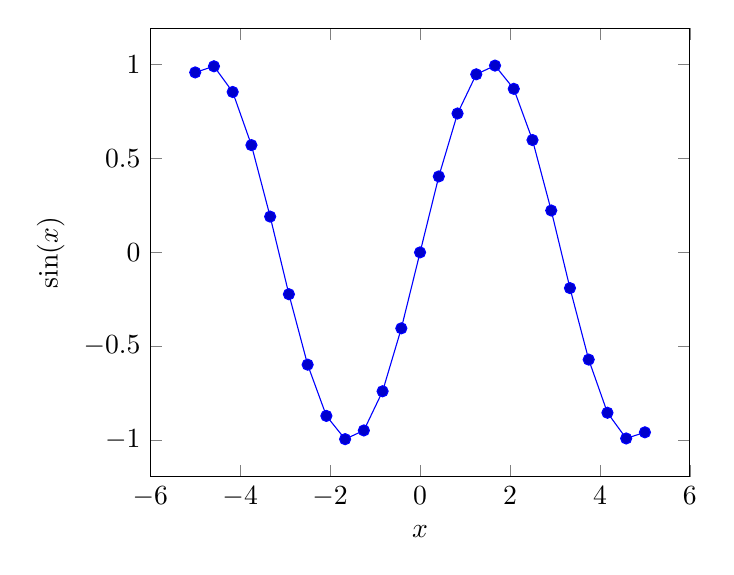
\begin{tikzpicture}
        \begin{axis}[xlabel=$x$,
            ylabel=$\sin(x)$]
          \addplot {sin(deg(x))};  % Print sine function
        \end{axis}
      \end{tikzpicture}
    \end{center}
    \caption{Plot of $\sin(x)$ direclty inside the figure environment with pgfplots.}
  \end{figure}

  \begin{figure}[h]
    \begin{center}
      \begin{tikzpicture}
        \begin{axis}[xlabel=$x$,
            ylabel=$y$]
          \addplot table [x=a, y=c, col sep=comma] {data/data.csv};  % Read coordinates from csv file and plot them
        \end{axis}
      \end{tikzpicture}
    \end{center}
    \caption{Coordinates $x$ and $y$ read from csv file and plotted pgfplots.}
  \end{figure}

}{}


%%%%%%%%%%%%%%%%%%%%%%%%%%%%%%%%%%%%%%%%%%%%%%%%%%%%%%%%%%%%%%%%%%%%%%%%%%%%%%
\section{Figures with tikz}
%%%%%%%%%%%%%%%%%%%%%%%%%%%%%%%%%%%%%%%%%%%%%%%%%%%%%%%%%%%%%%%%%%%%%%%%%%%%%%
The tikz is a package for creating graphics programmatically. With this package grids or other regular strucutres can be easliy generated.

\begin{figure}[ht]
  \begin{center}
    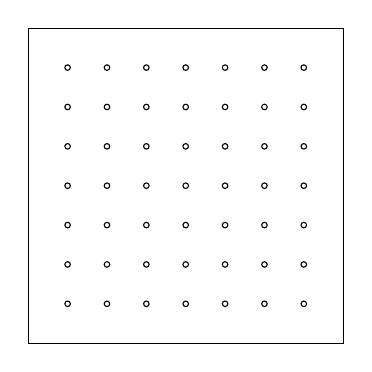
\begin{tikzpicture}
      \draw(0,0) rectangle (4,4);
      \foreach \x in {0.5,1,1.5,2,2.5,3,3.5}
      \foreach \y in {0.5,1,1.5,2,2.5,3,3.5}
      \draw(\x,\y) circle (1pt);
    \end{tikzpicture}
  \end{center}
  \caption{A regular grid genrated with easily with two for loops.}\label{fig:tikz_example}
\end{figure}


%%%%%%%%%%%%%%%%%%%%%%%%%%%%%%%%%%%%%%%%%%%%%%%%%%%%%%%%%%%%%%%%%%%%%%%%%%%%%%
\section{UML diagrams using tikz-uml}
%%%%%%%%%%%%%%%%%%%%%%%%%%%%%%%%%%%%%%%%%%%%%%%%%%%%%%%%%%%%%%%%%%%%%%%%%%%%%%

\Cref{fig:uml} presents a class diagram typeset using tikz-uml.

\begin{center}
\begin{figure}
\begin{tikzpicture}
\begin{umlpackage}{p}
\begin{umlpackage}{sp1}
\umlclass[template=T]{A}{
  n : uint \\ t : float
}{}
\umlclass[y=-3]{B}{
  d : double
}{
  \umlvirt{setB(b : B) : void} \\ getB() : B}
\end{umlpackage}
\begin{umlpackage}[x=10,y=-6]{sp2}
\umlinterface{C}{
  n : uint \\ s : string
}{}
\end{umlpackage}
\umlclass[x=2,y=-10]{D}{
  n : uint
  }{}
\end{umlpackage}

\umlassoc[geometry=-|-, arg1=tata, mult1=*, pos1=0.3, arg2=toto, mult2=1, pos2=2.9, align2=left]{C}{B}
\umlunicompo[geometry=-|, arg=titi, mult=*, pos=1.7, stereo=vector]{D}{C}
\umlimport[geometry=|-, anchors=90 and 50, name=import]{sp2}{sp1}
\umlaggreg[arg=tutu, mult=1, pos=0.8, angle1=30, angle2=60, loopsize=2cm]{D}{D}
\umlinherit[geometry=-|]{D}{B}
\umlnote[x=2.5,y=-6, width=3cm]{B}{A note with respect to class B}
\umlnote[x=7.5,y=-2]{import-2}{A anotation}
\end{tikzpicture}
\caption{Class diagram generated with tikz-uml. Example adapted from Nicolas Kielbasiewicz.}
\label{fig:uml}
\end{figure}
\end{center}

\section{UML diagrams using PlantUML}

In case \lualatex{} is used and PlantUML is installed, UML diagrams can be defined using PlantUML.

% Only works if "--shell-escape" is activated. Please activate only if you are sure, your compilation settings are correct
%\IfFileExists{plantuml.sty}{\input{latexhints-english-plantuml}}{}


%%%%%%%%%%%%%%%%%%%%%%%%%%%%%%%%%%%%%%%%%%%%%%%%%%%%%%%%%%%%%%%%%%%%%%%%%%%%%%
\section{Linguistic Forests}
%%%%%%%%%%%%%%%%%%%%%%%%%%%%%%%%%%%%%%%%%%%%%%%%%%%%%%%%%%%%%%%%%%%%%%%%%%%%%%

\begin{filecontents*}{\democodefile}
\begin{forest}
  [VP
    [DP]
    [V’
      [V]
      [DP]
    ]
  ]
\end{forest}
\end{filecontents*}
\PrintDemo{style=parallel}


%%%%%%%%%%%%%%%%%%%%%%%%%%%%%%%%%%%%%%%%%%%%%%%%%%%%%%%%%%%%%%%%%%%%%%%%%%%%%%
\section{Tables}
%%%%%%%%%%%%%%%%%%%%%%%%%%%%%%%%%%%%%%%%%%%%%%%%%%%%%%%%%%%%%%%%%%%%%%%%%%%%%%
\cref{tab:Ergebnisse} shows results and \cref{tab:Werte} shows how numerical data can be represented in a table.
\begin{table}
  \centering
  \begin{tabular}{ccc}
    \toprule
    \multicolumn{2}{c}{\textbf{summed}} & \textbf{Title}                                                          \\ \midrule
    Table                                      & as                                                           & in      \\
    \url{tabsatz.pdf}                            & recommended                                                     & gesetzt \\

    \multirow{2}{*}{Example}                    & \multicolumn{2}{c}{a nice example}                                \\
                                                 & \multicolumn{2}{c}{for using \qq{multirow}}           \\
    \bottomrule
  \end{tabular}
  \caption[Example Table]{Exampe Table -- see \url{http://www.ctan.org/tex-archive/info/german/tabsatz/}}
  \label{tab:Ergebnisse}
\end{table}

\begin{table}
  \centering
  \begin{tabular}{l *{8}{d{3.2}}}
    \toprule

                         & \multicolumn{2}{c}{\textbf{Parameter 1}} & \multicolumn{2}{c}{\textbf{Parameter 2}} & \multicolumn{2}{c}{\textbf{Parameter 3}} & \multicolumn{2}{c}{\textbf{Parameter 4}}                                                                                                                                       \\
    \cmidrule(r){2-3}\cmidrule(lr){4-5}\cmidrule(lr){6-7}\cmidrule(l){8-9}

    \textbf{Bedingungen} & \multicolumn{1}{c}{\textbf{M}}           & \multicolumn{1}{c}{\textbf{SD}}          & \multicolumn{1}{c}{\textbf{M}}           & \multicolumn{1}{c}{\textbf{SD}}          & \multicolumn{1}{c}{\textbf{M}} & \multicolumn{1}{c}{\textbf{SD}} & \multicolumn{1}{c}{\textbf{M}} & \multicolumn{1}{c}{\textbf{SD}} \\
    \midrule

    W                    & 1.1                                      & 5.55                                     & 6.66                                     & .01                                      &                                &                                 &                                &                                 \\
    X                    & 22.22                                    & 0.0                                      & 77.5                                     & .1                                       &                                &                                 &                                &                                 \\
    Y                    & 333.3                                    & .1                                       & 11.11                                    & .05                                      &                                &                                 &                                &                                 \\
    Z                    & 4444.44                                  & 77.77                                    & 14.06                                    & .3                                       &                                &                                 &                                &                                 \\
    \bottomrule
  \end{tabular}

  \caption{Example table for 4 constraints (W-Z), each having 4 parameters with (M und SD). Note: use always the same number of decimal places.}
  \label{tab:Werte}
\end{table}

\IfFileExists{pgfplotstable.sty}{

\subsection{Tables with pgfplots}
With the pgfplotstable package tables can be directly generated from a csv file.

\begin{table}[h]
\centering
\pgfplotstabletypeset[
col sep = comma,
every head row/.style={before row=\toprule,after row=\midrule},
every last row/.style={after row=\bottomrule},
display columns/0/.style={string type,column name={}}
]
{data/data.csv}
\caption{Table direclty generated from the values of a csf file.}
\end{table}
}{}


\section{Tables spanning multiple pages}


\begin{longtable}{|l|l|l|}
\caption{A sample long table.} \label{tab:long} \\

\hline \multicolumn{1}{|c|}{\textbf{First column}} & \multicolumn{1}{c|}{\textbf{Second column}} & \multicolumn{1}{c|}{\textbf{Third column}} \\ \hline
\endfirsthead

\multicolumn{3}{c}%
{{\bfseries \tablename\ \thetable{} -- continued from previous page}} \\
\hline \multicolumn{1}{|c|}{\textbf{First column}} & \multicolumn{1}{c|}{\textbf{Second column}} & \multicolumn{1}{c|}{\textbf{Third column}} \\ \hline
\endhead

\hline \multicolumn{3}{|r|}{{Continued on next page}} \\ \hline
\endfoot

\hline \hline
\endlastfoot

A & BC & D \\
A & BC & D \\
A & BC & D \\
A & BC & D \\
A & BC & D \\
A & BC & D \\
A & BC & D \\
A & BC & D \\
A & BC & D \\
A & BC & D \\
A & BC & D \\
A & BC & D \\
A & BC & D \\
A & BC & D \\
A & BC & D \\
A & BC & D \\
A & BC & D \\
A & BC & D \\
A & BC & D \\
A & BC & D \\
A & BC & D \\
A & BC & D \\
A & BC & D \\
A & BC & D \\
A & BC & D \\
A & BC & D \\
A & BC & D \\
A & BC & D \\
A & BC & D \\
A & BC & D \\
A & BC & D \\
A & BC & D \\
A & BC & D \\
A & BC & D \\
A & BC & D \\
A & BC & D \\
A & BC & D \\
A & BC & D \\
A & BC & D \\
A & BC & D \\
A & BC & D \\
A & BC & D \\
A & BC & D \\
A & BC & D \\
A & BC & D \\
A & BC & D \\
A & BC & D \\
A & BC & D \\
A & BC & D \\
A & BC & D \\
A & BC & D \\
A & BC & D \\
A & BC & D \\
A & BC & D \\
A & BC & D \\
A & BC & D \\
A & BC & D \\
A & BC & D \\
A & BC & D \\
A & BC & D \\
A & BC & D \\
A & BC & D \\
A & BC & D \\
A & BC & D \\
A & BC & D \\
A & BC & D \\
A & BC & D \\
A & BC & D \\
A & BC & D \\
A & BC & D \\
A & BC & D \\
A & BC & D \\
A & BC & D \\
A & BC & D \\
A & BC & D \\
A & BC & D \\
A & BC & D \\
A & BC & D \\
A & BC & D \\
A & BC & D \\
\end{longtable}


%%%%%%%%%%%%%%%%%%%%%%%%%%%%%%%%%%%%%%%%%%%%%%%%%%%%%%%%%%%%%%%%%%%%%%%%%%%%%%
\section{Abbreviations}
%%%%%%%%%%%%%%%%%%%%%%%%%%%%%%%%%%%%%%%%%%%%%%%%%%%%%%%%%%%%%%%%%%%%%%%%%%%%%%
At the first pass the \gls{fr} was 5.
At the second pass was \gls{fr} 3.
The plural form can be seen here: \glspl{er}.
To demonstrate what the list of abbreviations looks like for longer description texts, \glspl{rdbms} must be mentioned here.

With \verb+\gls{...}+ you can enter abbreviations, the first time you call it, the long form is used.
When reusing \verb+\gls{..}+ the short form is automatically displayed.
The abbreviation is also automatically inserted in the abbreviation list.
With \verb+\glspl{...}+ the plural form is used.
If you want the short form to appear directly at the first use, you can use \verb+\glsunset{..}+ to mark an abbreviation as already used.
The opposite is achieved with \verb+\glsreset{..}+.

Abbreviations are defined in \verb+\content\ausarbeitung.tex+ by means of \verb+\newacronym{...}{...}{...}+.

More information at: \url{http://tug.ctan.org/macros/latex/contrib/glossaries/glossariesbegin.pdf}
%%%%%%%%%%%%%%%%%%%%%%%%%%%%%%%%%%%%%%%%%%%%%%%%%%%%%%%%%%%%%%%%%%%%%%%%%%%%%%
\section{References}
%%%%%%%%%%%%%%%%%%%%%%%%%%%%%%%%%%%%%%%%%%%%%%%%%%%%%%%%%%%%%%%%%%%%%%%%%%%%%%
For distant sections \qq{varioref} is recommended:
\qq{See \vref{sec:mf}}.
The command \texttt{\textbackslash{}vref} works similar to \texttt{\textbackslash{}cref} the difference beeing that a reference to the page is additionally added.
\texttt{vref}: \qq{\vref{sec:firstsectioninlatexhints}}, \texttt{cref}: \qq{\cref{sec:firstsectioninlatexhints}}, \texttt{ref}: \qq{\ref{sec:firstsectioninlatexhints}}.

If \qq{varioref} causes difficulties, then \qq{cref} can be used instead.
This also creates the word \qq{section} automatically: \cref{sec:mf}.
This is also possible for illustrations etc.
In English please use \verb1\Cref{...}1 (with large \qq{C} at the beginning).

%With MiKTeX installation from 2012-01-16 no longer necessary.
%If a section becomes longer than one page and you want to refer to a specific place in the section with \texttt{\textbackslash{}vref}, then you should use \texttt{\textbackslash{}phantomsection} then using \texttt{vref} will also display the correct page number.

%%The link location will be placed on the line below.
%%Tipp von http://en.wikibooks.org/wiki/LaTeX/Labels_and_Cross-referencing#The_hyperref_package_and_.5Cphantomsection
%\phantomsection
%\label{alabel}
%View the example for \texttt{\textbackslash{}phantomsection} in the \LaTeX{} source code.

%Here is the example: See Section \vref{hack1} and Section \vref{hack2}.
%%%%%%%%%%%%%%%%%%%%%%%%%%%%%%%%%%%%%%%%%%%%%%%%%%%%%%%%%%%%%%%%%%%%%%%%%%%%%%
\section{Definitions}
%%%%%%%%%%%%%%%%%%%%%%%%%%%%%%%%%%%%%%%%%%%%%%%%%%%%%%%%%%%%%%%%%%%%%%%%%%%%%%
\begin{definition}[Title]
  \label{def:def1}
  Definition Text
\end{definition}

\Cref{def:def1} shows \ldots

%%%%%%%%%%%%%%%%%%%%%%%%%%%%%%%%%%%%%%%%%%%%%%%%%%%%%%%%%%%%%%%%%%%%%%%%%%%%%%
\section{Footnotes}
%%%%%%%%%%%%%%%%%%%%%%%%%%%%%%%%%%%%%%%%%%%%%%%%%%%%%%%%%%%%%%%%%%%%%%%%%%%%%%
Footnotes are provided by the command \verb+\footnote{...}+\footnote{\label{fussnote}Example footnote.}. Citing footnotes is possible by provinding a label\verb+\footnote{\label{...}...}+ and cite the footnote with \verb+\cref{...}+ in the text\cref{fussnote}.
%%%%%%%%%%%%%%%%%%%%%%%%%%%%%%%%%%%%%%%%%%%%%%%%%%%%%%%%%%%%%%%%%%%%%%%%%%%%%%

%%%%%%%%%%%%%%%%%%%%%%%%%%%%%%%%%%%%%%%%%%%%%%%%%%%%%%%%%%%%%%%%%%%%%%%%%%%%%%
\section{Various Things}
%%%%%%%%%%%%%%%%%%%%%%%%%%%%%%%%%%%%%%%%%%%%%%%%%%%%%%%%%%%%%%%%%%%%%%%%%%%%%%
\label{sec:diff}
\ifdeutsch
  Numbers (123\,654\,789) are nicely set.
  Either in a line or as non-lining figure.
  The latter is reached by parameter \texttt{osf} at package \texttt{libertine} or.\ \texttt{mathpazo} in \text{fonts.tex}.
\fi

\begin{filecontents*}{\democodefile}
\begin{compactenum}[I.]
  \item You can also keep the numbering compact thanks to paralist
  \item and switch to a different numbering
\end{compactenum}
\end{filecontents*}
\PrintDemo{style=parallel}

The words \qq{workflow} and \qq{dwarflike} can be copied from the PDF and pasted to a text file.

\begin{filecontents*}{\democodefile}
In case \LuaLaTeX{} is used as compiler, there is no ligature at \qq{f\/l} in the word \qq{dwarflike} (in contrast to \qq{fl} at \qq{workflow}).
In other words: \qq{dwarflike} and \qq{dwarf\/like} look the same in the PDF.
In case they do not, there is an issue with Lua\LaTeX{} and the selnolig package.
\end{filecontents*}
\PrintDemo{style=parallel}
% Meta comment: The precise form of the optimal ligation suppression command may vary depending on the character pairs involved - see https://tex.stackexchange.com/q/28437/9075


%%%%%%%%%%%%%%%%%%%%%%%%%%%%%%%%%%%%%%%%%%%%%%%%%%%%%%%%%%%%%%%%%%%%%%%%%%%%%%
\section{Closing remarks}
%%%%%%%%%%%%%%%%%%%%%%%%%%%%%%%%%%%%%%%%%%%%%%%%%%%%%%%%%%%%%%%%%%%%%%%%%%%%%%
Please feel free to provide enhancements for this template and create a new ticket on GitHub (\url{https://github.com/latextemplates/uni-stuttgart-computer-science-template/issues}).





\chapter{REMOVE THIS BEFORE HANDIN !!!!}

\section{Things to read(temp list)}

https://www.microsoft.com/en-us/research/wp-content/uploads/2016/02/tr-95-51.pdf

https://docs.microsoft.com/en-us/azure/service-fabric/service-fabric-reliable-services-reliable-collections


\end{document}
